%
% Cheatsheet based on https://github.com/jcjgraf/ETH-Resources/tree/main/21-1_AMR-CS
%


% Basic stuff
\documentclass[a4paper]{article}
\usepackage[nswissgerman]{babel}
\usepackage{lmodern}
\usepackage[fontsize=5pt]{fontsize}

% 5 column landscape layout with fewer margins
\usepackage{geometry}
\geometry{paper=a4paper,left=4.5mm, right=4.5mm, top=4.5mm, bottom=6mm, landscape, nohead, nofoot}
\usepackage{flowfram}
\ffvadjustfalse
\setlength{\columnsep}{1cm}
\Ncolumn{4}

\usepackage[dvipsnames]{xcolor}

% define nice looking boxes
\usepackage[many]{tcolorbox}

% a base set, that is then customised
\tcbset {
	base/.style={
		boxrule=0mm,
		leftrule=1mm,
		left=1.75mm,
		arc=0mm, 
		fonttitle=\bfseries, 
		colbacktitle=black!10!white, 
		coltitle=black, 
		toptitle=0.75mm, 
		bottomtitle=0.25mm,
		title={#1}
	}
}

\definecolor{color-amr}{RGB}{178, 99, 92}
\newtcolorbox{mainbox}[1]{
	colframe=color-amr, 
	base={#1}
}

\newtcolorbox{subbox}[1]{
	colframe=black!20!white,
	base={#1}
}

\usepackage[small,compact]{titlesec}

% Mathematical typesetting & symbols
\usepackage{amsthm, mathtools, amssymb} 
\usepackage{marvosym, wasysym}
\usepackage{cancel}
\allowdisplaybreaks
% \addtolength{\arraycolsep}{-4pt}

% algorithms
\usepackage{algorithmic}
\usepackage{algorithm}
\algsetup{linenodelimiter=}

% Tables
\usepackage{tabularx, multirow}
\usepackage{makecell}
\usepackage{booktabs}
% \renewcommand*{\arraystretch}{2}

% Make enumerations more compact
\usepackage[inline]{enumitem}
\setlist{nolistsep}
\setlistdepth{20}
\renewlist{itemize}{itemize}{20}
\setlist[itemize]{label=$\cdot$}
\setlist[itemize,1]{label=\textbullet}
\setlist[itemize,2]{label=--}
\setlist[itemize,3]{label=$\ast$}
\setlist[itemize,4]{label=$\circ$}
\setlist[itemize,5]{label=$\triangleright$}
\setlist[itemize,6]{label=$\diamond$}
\setitemize{leftmargin=0.2cm}
\newcommand{\ipro}{\item[+]}
\newcommand{\icon}{\item[-]}
\newcommand{\ides}[1]{\item \textbf{#1}}

% To include sketches & PDFs
\usepackage{graphicx}

% For hyperlinks
\usepackage{hyperref}
\hypersetup{
	colorlinks=true
}

% Metadata
\title{Cheatsheet\\ Autonomous Mobile Robots}
\author{Florian Affolter}
\date{\vspace{-10pt}Sommersession 2024}

% Start with section 0
\setcounter{section}{-1}

% Math helper stuff
\def\limxo{\lim_{x\to 0}}
\def\limxi{\lim_{x\to\infty}}
\def\limxn{\lim_{x\to-\infty}}
\def\R{\mathbb{R}}
\def\P{\mathbb{P}}
\def\F{\mathcal{F}}
\def\E{\mathbb{E}}
\DeclareMathOperator{\Var}{\text{Var}}

\newcommand{\norm}[1]{\left| \!\:\! \left| #1 \right| \!\:\! \right|}
\newcommand{\transpose}{\mathsf{T}}
\newcommand{\rmd}{\mathrm{d}}
\newcommand{\bigO}{\mathcal{O}}

\raggedright


\begin{document}

% \maketitle

% \input{../license.tex}


\section{General}
\begin{itemize}
    \item $\mathrm{cov}(X, Y) = E((X - E(X))(Y - E(Y)))$
    \ides{Covariance $\mathbf{C}$:} $C_{X_i,X_j} = \mathrm{cov}(X_i, X_j)$
        \\ \begin{itemize*}
            \item Square
            \item Diagonal is variance
        \end{itemize*}
    \ides{Cond. P.:} $P[B | A] := \frac{P[B \cap A]}{P[A]}$
    \ides{Tot. P.:} $P[B] = \sum_{i=1}^n P[B \mid A_i] \cdot P[A_i]$
    \ides{Bayes:} $P[A \mid B] = \frac{P[B \mid A]\cdot P[A]}{P[B]}$
    \ides{Indep.:} $P[A \cap B] = P[A] \cdot P[B]$
    \item $E[X] = \int_{-\infty}^{\infty} x f_X(x) \mathrm{d}x$
    \item $Var[X] = E[(X - E[X])^2]$
    \item Cartesian $(x, y) \Leftrightarrow$ Polar $(r, \varphi)$
        \begin{itemize}
            \item
                \begin{itemize*}
                    \item $x = r \cos(\varphi)$
                    \item $y = r \sin(\varphi)$
                \end{itemize*}
            \item
                \begin{itemize*}
                    \item $r = \sqrt{x^2 + y^2}$
                    \item $\cos(\varphi) = \frac{x}{r}$
                    \item $\sin(\varphi) = \frac{y}{r}$
                \end{itemize*}
        \end{itemize}
\end{itemize}


\section{Introduction}
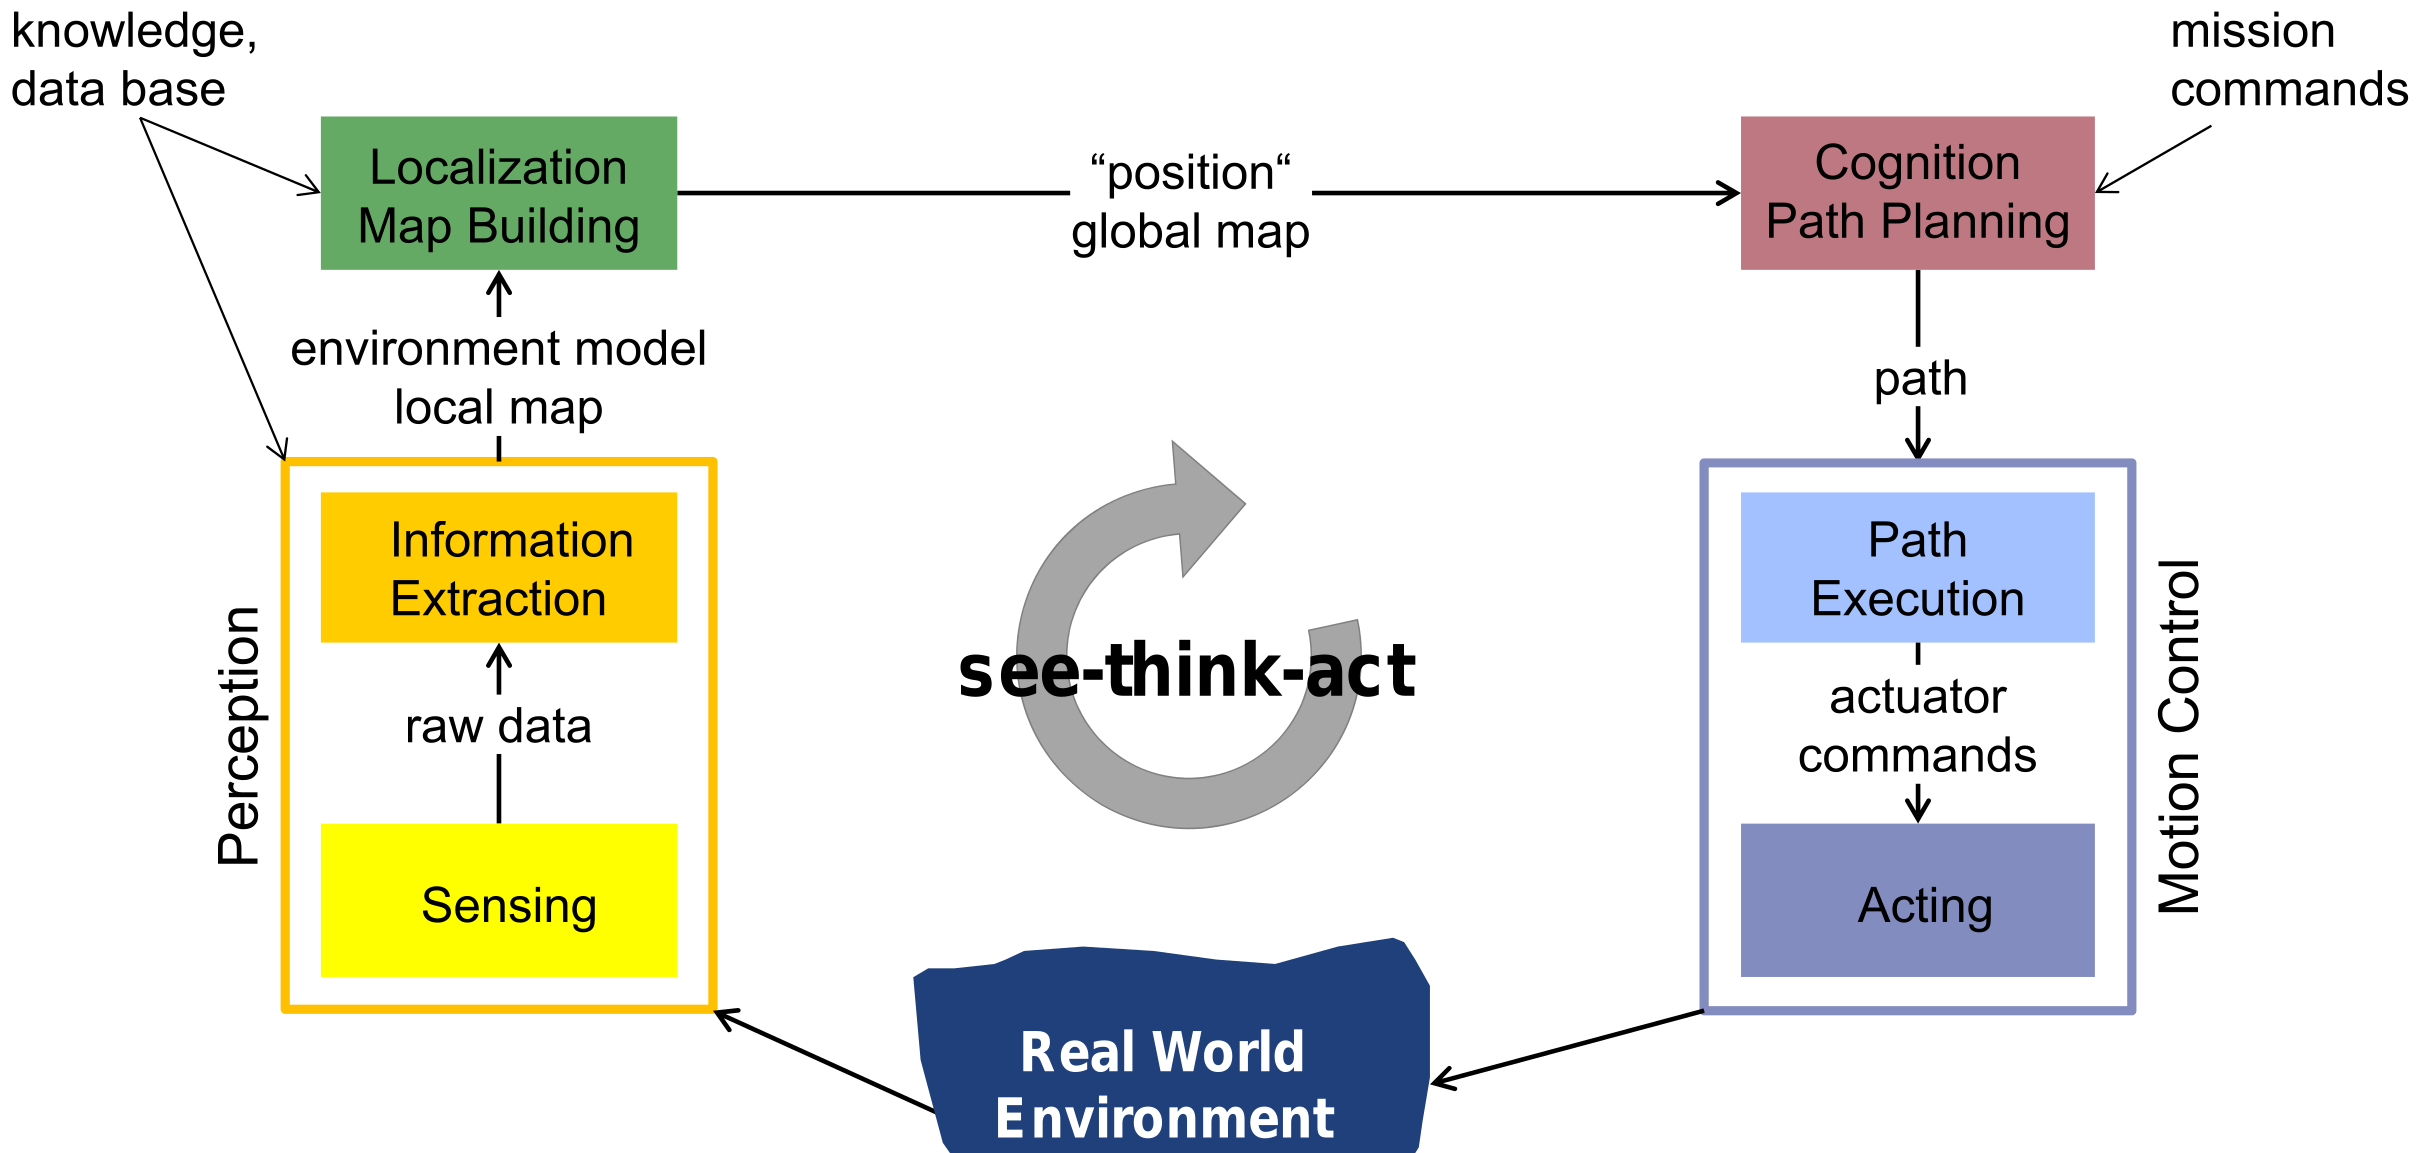
\includegraphics[width=\linewidth]{./Figures/01_SeeThinkAct.png}


\section{Locomotion}
\begin{itemize}
    \item Physical interaction between vehicle and environment
    \ides{Stability:} characterized by
        \begin{itemize*}
            \item Number of contact pts
            \item CoG
            \item Static/dynamic stabilization
            \item Inclination of terrain
        \end{itemize*}
    \ides{Contact:} characterized by
        \begin{itemize*}
            \item Contact pt size and shape
            \item Angle of contact
            \item Friction
        \end{itemize*}
    \ides{Environment:} characterized by
        \begin{itemize*}
            \item Structure
            \item Medium
        \end{itemize*}
    \ides{Implementation Aspects:}
        \begin{itemize*}
            \item Number of actuators
            \item Structural complexity
            \item control complexity
            \item Energy consumption
        \end{itemize*}
        \ides{Cost of transportation $C_{mt}$:} $= \frac{E}{m \cdot g \cdot d} = \frac{P}{m \cdot g \cdot v}$,
        \begin{itemize*}
            \ides{E:} Energy
            \ides{P:} Power
            \ides{m:} Mass
            \ides{d:} Distance
            \ides{v:} Speed
        \end{itemize*}
\end{itemize}

\subsection{Legged Locomotion}
\begin{itemize*}
    \ipro Mobility
    \ipro Adaptability
    \ipro Ability to manipulate environment
    \icon Mechanical complexity
    \icon Control complexity
    \icon Energy Consumption
\end{itemize*}
\begin{itemize}
    \ides{Gait:} Distinct sequence of lift and release events of individual legs
    \item $\#$ possible events for $k$ legged robot is $N = (2k - 1)!$
    \ides{Static Gaits:}
        \begin{itemize*}
            \item System is statically sable
            \item Requires $\ge 4$ legs
            \ipro Safe
            \icon Slow
            \icon Energetically inefficient
        \end{itemize*}
    \ides{Dynamic Gaits:}
        \begin{itemize*}
            \item System is stabilized on a limited cycle
            \item Falls over if stopped
            \ipro Fast
            \ipro Energetically efficient
            \icon Demanding for actuators
            \icon Demanding for control
        \end{itemize*}
    \ides{Locomotion Control}
        \begin{itemize}
            \item[1)] Stepping sequence defined by gait pattern
            \item[2)] Stepping location
            \item[3)] Contact forces
        \end{itemize}
\end{itemize}

\subsection{Wheeled Locomotion}
\begin{itemize*}
    \ipro Highly efficient on flat surface
\end{itemize*}

\subsubsection{Wheel Types}
\begin{itemize}
    \ides{Standard Wheel:}
        \begin{itemize*}
            \item $2$ DoF
                (\begin{itemize*}
                    \item wheel axle
                    \item wheel contact point
                \end{itemize*})
            \item Can be steered or fixed
            \item Steering without side effects on the body
        \end{itemize*}
    \ides{Castor Wheel:}
        \begin{itemize*}
            \item $3$ DoF
                (\begin{itemize*}
                    \item wheel axle
                    \item wheel contact point
                    \item offset steering joint
                \end{itemize*})
            \item Steering must be compensated by the body
        \end{itemize*}
    \ides{Swedish Wheel:}
        \begin{itemize*}
            \item $3$ DoF
                (\begin{itemize*}
                    \item Rotation around the wheel axle
                    \item Rotation around the contact point
                    \item Rotation around the rollers
                \end{itemize*})
            \item Similar to standard wheel but provides low resistance in another direction
        \end{itemize*}
    \ides{Spherical Wheel:}
        \begin{itemize*}
            \item $3$ DoF
            \icon Difficult to realize
        \end{itemize*}
\end{itemize}

\subsubsection{Wheel Arrangements}
\begin{itemize}
    \item Influences manoeuvrability, controllability and stability
    \item No optimal arrangement
    \ides{Stability:}
        \begin{itemize*}
            \item $\ge 3$ wheels required for static stability
            \item Improved by adding more wheels
        \end{itemize*}
    \ides{Manoeuvrability:}
        \begin{itemize*}
            \item Number of DoF
        \end{itemize*}
    \ides{Controllability:}
        \begin{itemize*}
            \item Inverse correlation between controllability and manoeuvrability
            \item Less manoeuvrability robots can be controlled more accurately
        \end{itemize*}
\end{itemize}


\section{Kinematics}
% \subsection{Rigid Body Kinematics}
% \begin{minipage}[b]{0.43\linewidth}
%     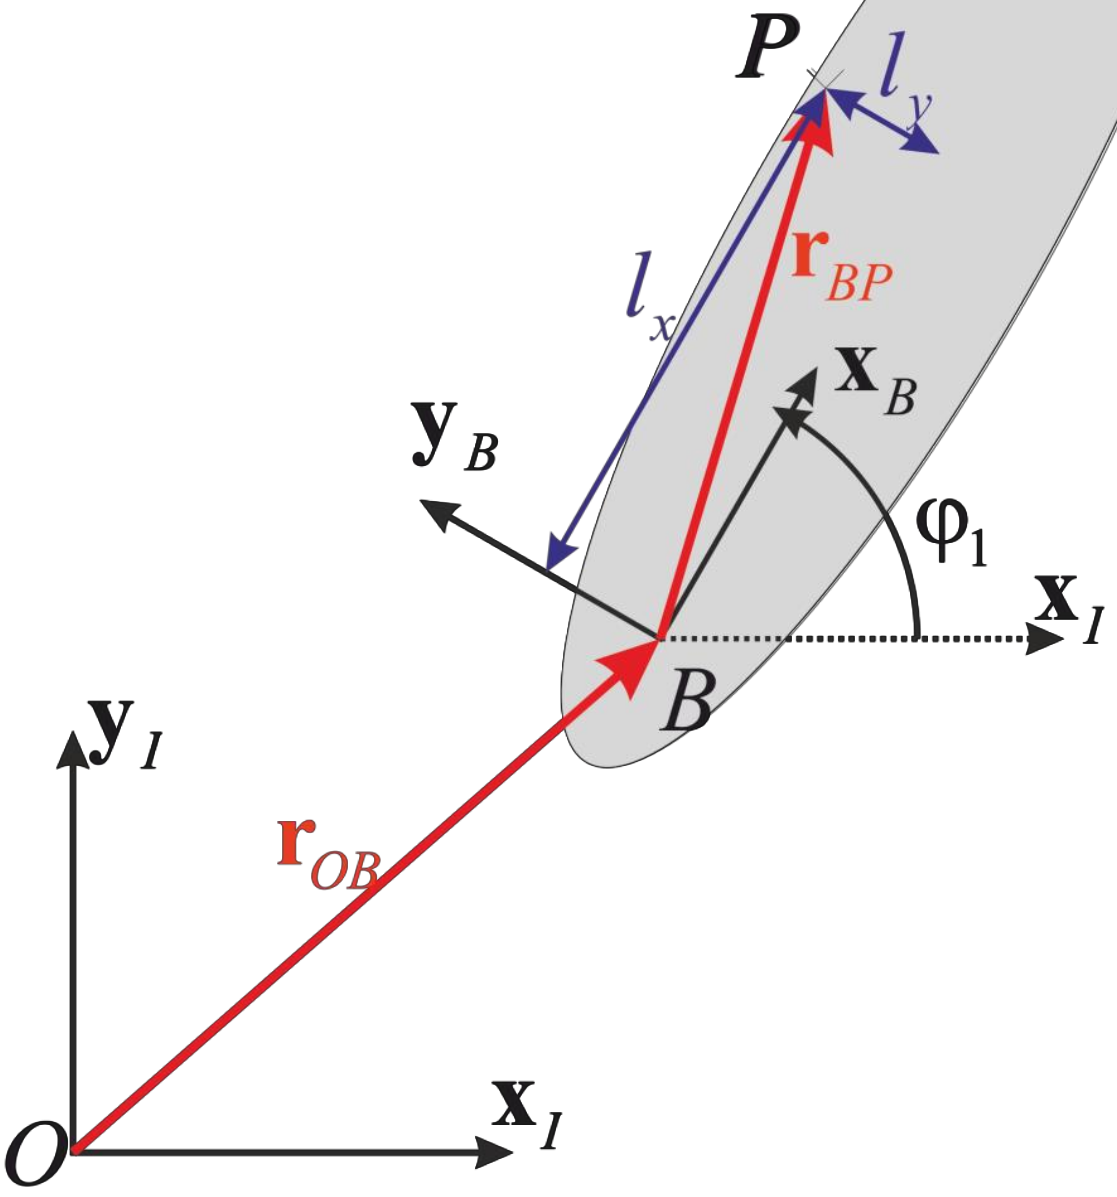
\includegraphics[width=\linewidth]{./Figures/03_RigidBodyTransformation.png}
% \end{minipage}
% \begin{minipage}[b]{0.55\linewidth}
%     \raggedright
%     \begin{itemize}
%         \ides{Translation:} All pts of the body move parallele
%             \begin{itemize}
%                 \item Vector from $O$ to $P$ in $I$: ${}_I r_{OP} = {}_I r_{OB} + {}_I r_{BP}$
%                 \item Velocity of of pt $P$ in $I$: ${}_I v_P = {}_I \dot r_{OP}$
%             \end{itemize}
%     \end{itemize}
% \end{minipage}
% \begin{itemize}
%         \ides{Rotation:} One pt is fixed an all other move around it
%             \begin{itemize}
%                 \item Vector $r$ in $B$ rotated to $I$: ${}_I r = R_{IB} {}_B r$
%                 \item Rotation $R_{IB}$ along $x, y, z$:
%                     $\begin{bmatrix}
%                         1 & 0 & 0\\
%                         0 & \cos(\varphi) & -\sin(\varphi)\\
%                         0 & \sin(\varphi) & \cos(\varphi)
%                     \end{bmatrix}$
%                     $\begin{bmatrix}
%                         \cos(\varphi) & 0 & \sin(\varphi)\\
%                         0 & 1 & 0\\
%                         - \sin(\varphi) & 0 & \cos(\varphi)\\
%                     \end{bmatrix}$
%                     $\begin{bmatrix}
%                         \cos(\varphi) & -\sin(\varphi) & 0\\
%                         \sin(\varphi) & \cos(\varphi) & 0\\
%                         0 & 0 & 1
%                     \end{bmatrix}$
%                 \ides{Inverse:} $R_{BI} = R^{-1}_{IB} = R^\transpose_{IB}$
%             \ides{Composition:} $R_{AI} = R_{AB} \cdot R_{BI}$
%             \item Angular velocity of $B$ in $I$ along $z$: ${}_I \omega_{IB} = (0, 0, \dot \varphi)^\transpose$
%                 \begin{itemize}
%                     \item Equal for every point in the body
%                 \end{itemize}
%             \ides{Transformation:} ${}_I \omega_{IB} = R_{IB} \ {}_B \omega_{IB}$
%             \ides{Composition:} ${}_I \omega_{IC} = {}_I \omega_{IB} + {}_I \omega_{BC}$
%             \item ${}_I \hat \omega_{IB} = \dot R_{IB} R^\transpose_{IB} =
%                 \begin{bmatrix}
%                     0 & -{}_I \omega^z_{IB} & {}_I \omega^y_{IB}\\
%                     {}_I \omega^z_{IB} & 0 & -{}_I \omega^x_{IB}\\
%                     -{}_I \omega^y_{IB} & {}_I \omega^x_{IB} & 0
%                 \end{bmatrix}, {}_I \omega_{IB} =
%                 \begin{bmatrix}
%                     {}_I \omega^x_{IB}\\
%                     {}_I \omega^y_{IB}\\
%                     {}_I \omega^z_{IB}
%                 \end{bmatrix}$
%         \end{itemize}
%     \ides{Homogeneous Transformation:} Rotation $+$ Translation
%         \begin{itemize}
%             \item Vector from $O$ to $P$ in $I$: ${}_I r_{OP} = {}_I r_{OP} + R_{IB} \ {}_B r_{BP}$
%             \item $
%                 \begin{pmatrix}
%                     {}_I r_{OP}\\
%                     1
%                 \end{pmatrix} =
%                 \begin{bmatrix}
%                     R_{IB} & {}_I r_{OB}\\
%                     0 & 1
%                 \end{bmatrix}
%                 \begin{pmatrix}
%                     {}_B r_{BP}\\
%                     1
%                 \end{pmatrix}$
%             \item Full motion: ${}_I v_P = {}_I \dot r_{OP} = {}_I \dot r_{OB} + {}_I \omega_{IB} \times {}_I r_{BP}$
%         \end{itemize}
%     \ides{Vector Differentiation}
%         \begin{itemize}
%             \ides{Non-moving system:} ${}_I r \implies {}_I \dot r = \frac{d {}_I r}{dt}$
%             \ides{Moving (translating or rotating) system:} ${}_B r \implies {}_B \dot r = \frac{d {}_B r}{dt} + {}_B \omega_{IB} \times {}_B r$
%         \end{itemize}
%     \ides{Generalized Coordinated}
%         \begin{itemize}
%             \item Set of independent variables that uniquely describe the robot's configuration
%             \item $q = (q_1, q_2, \dots q_n)^\transpose$
%             \item ${}_I r_{OP} = {}_I r_{OP}(q)$
%         \end{itemize}
%     \ides{Jacobians}
%         \begin{itemize}
%             \item $J_P = \frac{\partial r_{OP}(q)}{\partial q} =
%                 \begin{bmatrix}
%                     \frac{\partial r_1}{\partial q_1} & \dots & \frac{\partial r_1}{\partial q_n}\\
%                     \vdots & \ddots & \vdots\\
%                     \frac{\partial r_m}{\partial q_1} & \dots & \frac{\partial r_1}{\partial q_n}\\
%                 \end{bmatrix}$
%             \item Cartesian velocity to generalized velocity: $\dot r_P = J \dot q$
%             \item Change in generalized coordinates to Cartesian space: $\bigtriangleup r_P = J \bigtriangleup q$
%         \end{itemize}
% \end{itemize}

\subsection{Inverse Kinematics}
\begin{itemize}
    \item Given desired endeffector position $r_{OF}(q) = r^{\text{goal}}_{OF}$, determine generalized coordinates $q$
    \item $r_{OF}(q)$ not easily invertible
\end{itemize}
\begin{minipage}[b]{0.6\linewidth}
    \begin{itemize}
        \ides{Iterative Method:}
            \begin{itemize}
                \item[1)] Initialize $q = q^0$ to initial guess and set $r = r(q)$
                \item[2)] Evaluate Jacobian $J_P = \left.\frac{\partial r_{OF}}{\partial q} \right|_{q = q^i}$
                \item[3)] Invert Jacobian to obtain $\bigtriangleup q = J^+ \bigtriangleup r_{OF}$
                \item[4)] Update generalized coordinates $q^{i+1} = q^i + J^+(r^\text{goal}_{OF} - r^j_{OF}$
                \item[5)] Repeat from $2$ till converge
            \end{itemize}
    \end{itemize}
\end{minipage}
\begin{minipage}[b]{0.38\linewidth}
    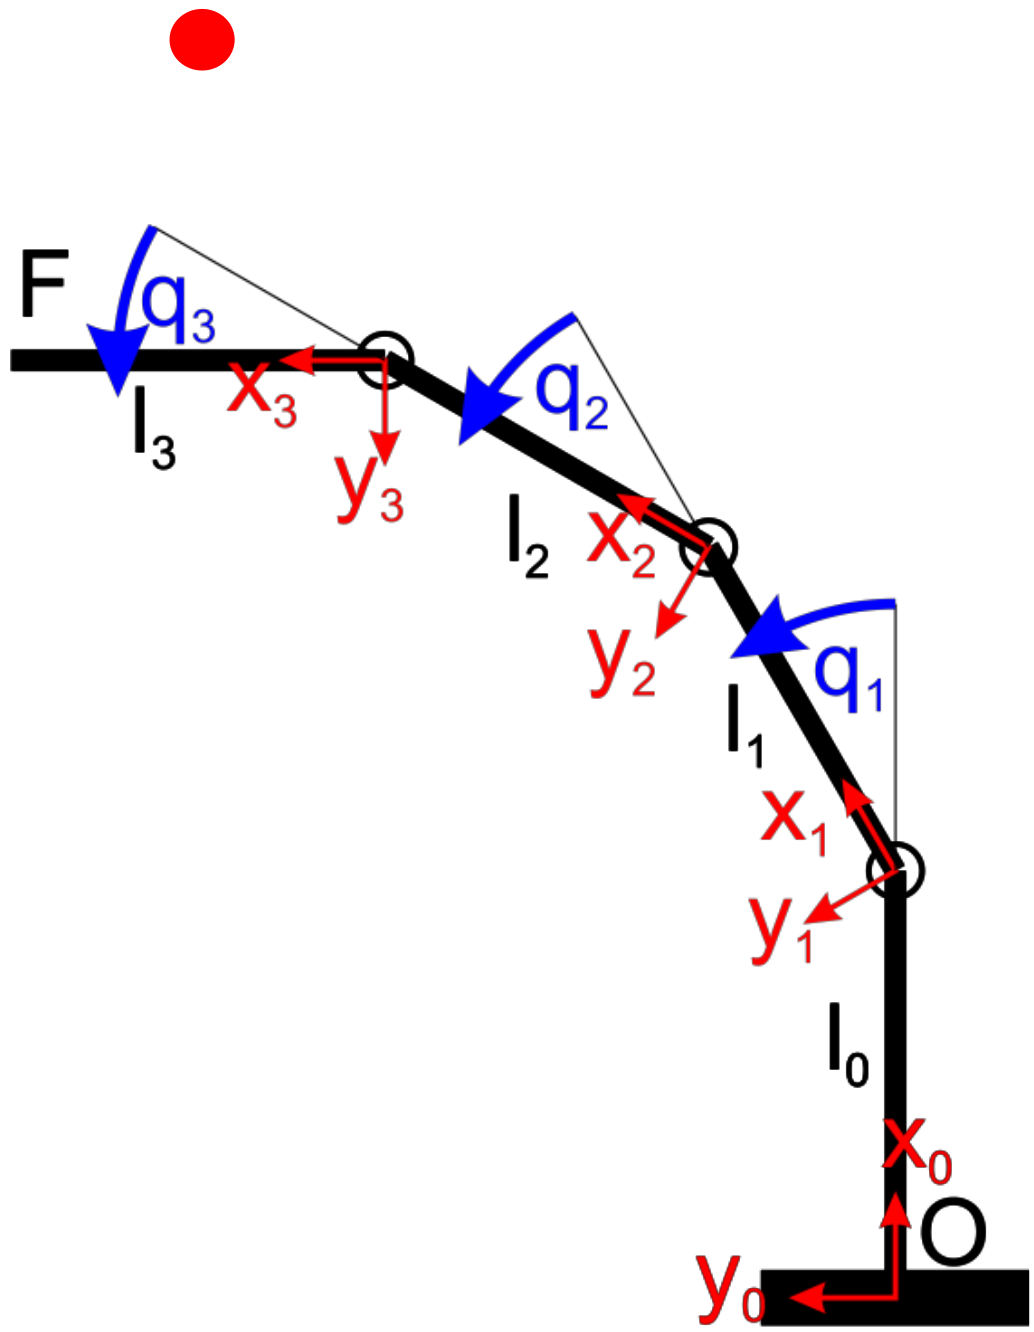
\includegraphics[width=\linewidth]{./Figures/03_InverseKinematrics.png}
\end{minipage}

\subsection{Inverse Differential Kinematics}
\begin{itemize}
    \item Given desired endeffector velocity $\dot r_{F} = J_P \dot q = r^\text{goal}_F$, determine generalized velocity $q = J^+_P \dot r^\text{goal}_F$
\end{itemize}

\subsection{Redundancy and Singularity}
\begin{itemize}
    \ides{Redundancy:} Jacobian is column-rank deficient
        \begin{itemize}
            \item Pseudo inverse minimizes $\norm{\dot q}_2$
            \item Can have multiple solutions $\dot q = J^+ \dot r^\text{goal} + \underbrace{(I - J^+ J)}_{N} \dot q_0$
            \item $q_0$ is chosen solution
        \end{itemize}
    \ides{Singularity:} Jacobian is row-rank deficient
        \begin{itemize}
            \item Pseude inverse minimizes error $\norm{\dot r^\text{goal} - \dot r}_2$
        \end{itemize}
\end{itemize}

\subsection{Mobile Robot Kinematics}
\begin{itemize}
    \ides{Legged Robot:} Quadropod
        \begin{itemize}
            \item $q =
                \begin{bmatrix}
                    q_B\\
                    q_r
                \end{bmatrix}
                \begin{matrix}
                    \text{Un-actuated base}\\
                    \text{Actuated joints}
                \end{matrix}$
            \ides{Contact Constraint:} $\dot r_F = J_F \dot q = 0 \Rightarrow \dot q = \cancel{J^+_F \dot r_F}^{=0} + N_F \dot q_0$
            \ides{Body Move:} $\dot r_B = J_B \dot q = J_B N_F \dot q_0$
        \item $\dot q = \cancel{J^+_F \dot r_F}^{=0} + N_F \dot q_0 = N_F(J_B N_F)^+ \dot r_B$
        \end{itemize}
    \ides{Wheeled Robot:} Planar car
        \begin{itemize}
            \item $q =
                \begin{bmatrix}
                    x\\
                    \varphi
                \end{bmatrix}$
            \item Point on wheel: ${}_I r_{OP} =
                \begin{bmatrix}
                    x + r \sin(\varphi)\\
                    r + r \cos(\varphi)\\
                        0
                \end{bmatrix}$
            \item ${}_I J_P =
                \begin{bmatrix}
                    1 & r \cos(\varphi)\\
                    0 & -r \sin(\varphi)\\
                    0 & 0
                \end{bmatrix}$
        \ides{Contact Constraint:} $\left. {}_I \dot x_P \right|_{\varphi = \pi} = \left. {}_I J_P \right|_{\varphi = \pi} \dot q =
                    \begin{bmatrix}
                        1 & -r\\
                        0 & 0\\
                        0 & 0
                    \end{bmatrix}
                    \begin{bmatrix}
                        \dot x\\
                        \dot \varphi
                    \end{bmatrix} = 0$
            \ides{Rolling Constraint:} $\dot x - r \dot \varphi = 0$
        \end{itemize}
\end{itemize}

\subsection{Mobile Robots}
\begin{itemize}
    \ides{Holonomic:}
        \begin{itemize*}
            \item Can move instantaneously in any direction of its DoF
            \item Differential constraints are integrable
        \end{itemize*}
    \ides{Non-Holonomic:}
        \begin{itemize*}
            \item Cannot move instantaneously in any direction of its DoF
            \item Differential constraints are not integrable
        \end{itemize*}
    \ides{Differential Forward Kinematics:} Given set of actuator speeds, determine its corresponding velocity
    \ides{Differential Inverse Kinematics:} given a desired velocity, determine the corresponding actuator speeds
\end{itemize}

\subsubsection{Wheel Kinematic}
\begin{minipage}[b]{0.48\linewidth}
    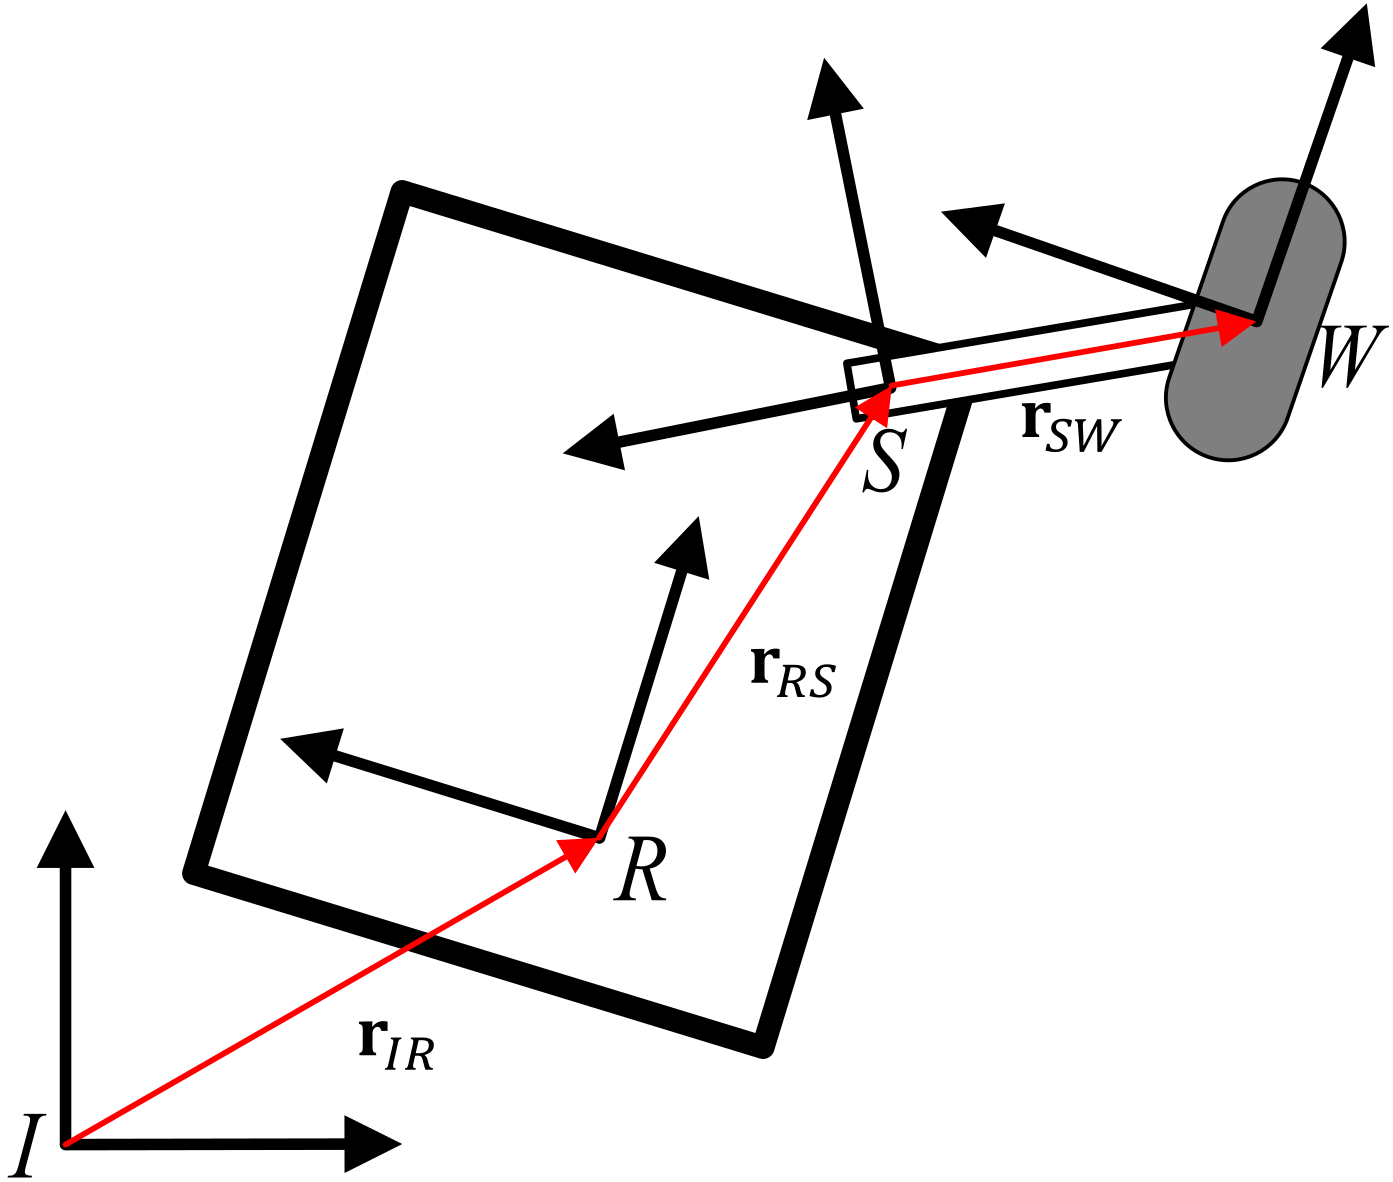
\includegraphics[width=\linewidth]{./Figures/03_WheelEquation.png}
\end{minipage}
\begin{minipage}[b]{0.48\linewidth}
    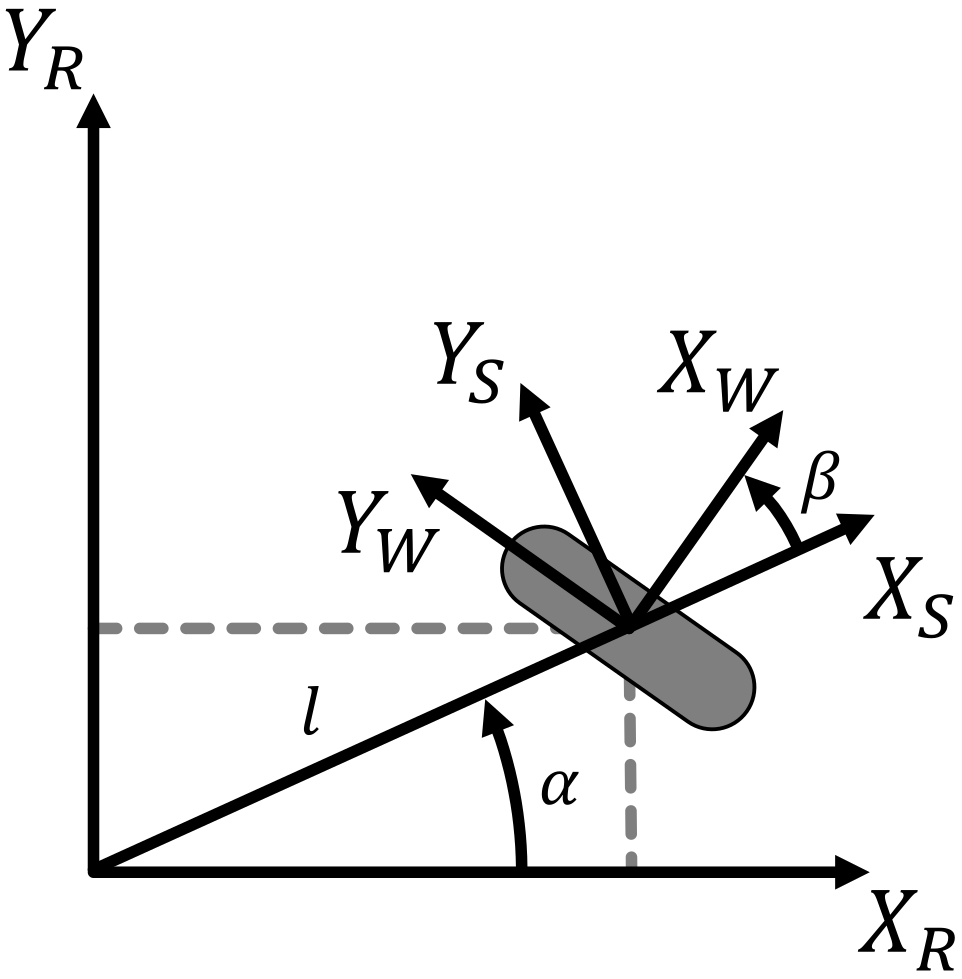
\includegraphics[width=\linewidth]{./Figures/03_StandardWheel.png}
\end{minipage}

\begin{itemize*}
    \item Robot state: $\xi_I = [x, y, \theta]^\transpose$
    \item $\dot \xi_I = [\dot x, \dot y, \dot \theta]^\transpose$
    \item $\dot \xi_R = R(\theta) \dot \xi_I$
    \item $R(\theta) = R^\transpose_z(\theta)$
\end{itemize*}
\begin{itemize}
    \item ${}_W v_{IW} =
        \begin{bmatrix}
            0\\
            -r \dot \varphi\\
            0
        \end{bmatrix}
        \begin{matrix}
            \text{no-sliding constraint}\\
            \text{rolling constraint}\\
            \text{planar assumption}
        \end{matrix}$
    \ides{Rolling Constraint:} $J_1(\beta_s) R(\theta) \dot \xi_I - \dot \varphi r = 0$
    \ides{No-Sliding Constraint:} $C_1(\beta_s) R(\theta) \dot \xi_I = 0$
    \ides{General Wheel Equation:} $v_{IW} = v_{IR} + \omega_{IR} \times r_{RS} + \omega_{IR} \times r_{SW} + \omega_{RS} \times r_{SW}$
    \ides{Standard (Steered \& Fixes) Wheel:} $r_{SW} = 0$
        \begin{itemize}
            \ides{Wheel Equation:} $v_{IW} = v_{IR} + \omega_{IR} \times r_{RS}$
                \begin{itemize}
                    \item ${}_W v_{IR} = R(\alpha + \beta) R(\theta)[\dot x, \dot y, 0]^\transpose$
                    \item ${}_W \omega_{IR} \times {}_W r_{RS} = [l \dot \theta \sin(\beta), l \dot \theta \cos(\beta), 0]^\transpose$
                \end{itemize}
            \item $J_1(\beta_s) = [\sin(\alpha + \beta_s), -\cos(\alpha + \beta_s), -l \cos(\beta_s)]$
            \item $C_1(\beta_s) = [\cos(\alpha + \beta_s), \sin(\alpha + \beta_s), l \sin(\beta_s)]$
            \item If fixed, $J_1(\beta_s) = J_1, C_1(\beta_s) = C_1$
            \item Only wheel which imposes constraints
        \end{itemize}
    \ides{Castor Wheel:}
        \begin{itemize}
            \item $J_1(\beta_s)$ same as standard wheel
            \item $C_1(\beta_s) = [\cos(\alpha + \beta_s), \sin(\alpha + \beta_s), d + l \sin(\beta)]$
        \end{itemize}
    \ides{Swedish Wheel:}
        \begin{itemize}
            \item $J_1(\beta_s) = [\sin(\alpha + \beta_s + \gamma), -\cos(\alpha + \beta_s + \gamma), -l \cos(\beta_s + \gamma)]$
            \item $C_1(\beta_s) = [\cos(\alpha + \beta_s + \gamma), \sin(\alpha + \beta_s + \gamma), l \sin(\beta_s + \gamma)]$
        \end{itemize}
\end{itemize}

\subsubsection{Mobile Robot Kinematic}
\begin{itemize}
    \item $N = (N_f + N_s)$ wheeled robot
\end{itemize}
\begin{itemize*}
    \item $J_1(\beta_s) =
        \begin{bmatrix}
            J_{1f}\\
            J_{1S}(\beta_s)
        \end{bmatrix}$
    \item $C_1(\beta_s) =
        \begin{bmatrix}
            C_{1f}\\
            C_{1S}(\beta_s)
        \end{bmatrix}$
    \item $J_2 = \mathrm{diag}(r_1, \dots, r_N)$
    \item $\dot \varphi =
        \begin{bmatrix}
            \dot \varphi_f\\
            \dot \varphi_s
        \end{bmatrix}$
\end{itemize*}
\begin{itemize}
    \ides{Rolling Constraint:} $J_1(\beta_s) R(\theta) \dot \xi_I - J_2 \dot \varphi = 0$
    \ides{No-Sliding Constraint:} $C_1(\beta_s) R(\theta) \dot \xi_I = 0$
    \item $
        \underbrace{\begin{bmatrix}
            J_1(\beta_s)\\
            C_1(\beta_s)
        \end{bmatrix}}_{A} \underbrace{R(\theta) \dot \xi_I}_{\dot \xi_R} =
        \underbrace{\begin{bmatrix}
            J_2\\
            0
        \end{bmatrix}}_{B} \dot \varphi$
    \ides{Forward Kinematics:} $\dot \xi_R = (A^\transpose A)^{-1} A^\transpose B \dot \varphi = A^+ B \dot \varphi$
    \ides{Inverse Kinematics:} $\dot \varphi = (B^\transpose B)^{-1} B^\transpose A \dot \xi_R = B^+ A \dot \varphi$
    \ides{Differential Drive:}
        \begin{itemize*}
            \item $\alpha_r = -\pi / 2$
            \item $\beta_r = \pi$
            \item $l_r = b$
            \item $r_r = r$
            \item $\alpha_r = \pi / 2$
            \item $\beta_r = 0$
            \item $l_l = -b$
            \item $r_l = r$
            \item $
                \begin{bmatrix}
                    \dot x\\
                    \dot y\\
                    \dot \theta
                \end{bmatrix}_R =
                \begin{bmatrix}
                    r / 2 & r / 2\\
                    0 & 0\\
                    r / 2b & -r / 2b
                \end{bmatrix}
                \begin{bmatrix}
                    \dot \varphi_r\\
                    \dot \varphi_l
                \end{bmatrix}$
            \item $
                \begin{bmatrix}
                    \dot \varphi_r\\
                    \dot \varphi_l
                \end{bmatrix} =
                \begin{bmatrix}
                    1 / r & 0 & b / r\\
                    1 / r & 0 & -b / r
                \end{bmatrix}
                \begin{bmatrix}
                    \dot x\\
                    \dot y\\
                    \dot \theta
                \end{bmatrix}_R$
        \end{itemize*}
\end{itemize}

\subsubsection{Maneuverability}
\begin{itemize}
    \ides{Degree of Maneuverability $\mathbf{\delta_M}$} $= \delta_m + \delta_s$
    \ides{Degree of Mobility $\mathbf{\delta_m}$:} $= \mathrm{dim} \; N(C_1(\beta_S)) = 3 - \mathrm{rank}(C_1(\beta_s))$
        \begin{itemize*}
            \item $0 \le \delta_m \le 3$
            \item $\delta_m = 0 \Rightarrow N_f = N_s = 0$
            \item $\delta_m = 3 \Rightarrow$ motion not possible
        \end{itemize*}
    \ides{Degree of Steerability $\mathbf{\delta_s}$:} $= \mathrm{rank}(C_{1s}(\beta_s))$
        \begin{itemize*}
            \item $0 \le \delta_s \le 2$
            \item $\delta_s = 0 \Rightarrow N_s = 0$
            \item $\delta_s = 1 \Rightarrow N_s \ge 1$
            \item $\delta_s = 2 \Rightarrow N_f = 0$
        \end{itemize*}
    \ides{Examples (\( \delta_m + \delta_s = \delta_M \)):}
        \begin{itemize*}
            \item Omnidirectional: \( 3 + 0 = 3 \)
            \item Differential: \( 2 + 0 = 2 \)
            \item Omni-Steer: \( 2 + 1 = 3 \)
            \item Tricycle: \( 1 + 1 = 2 \)
            \item Two-Steer: \( 1 + 2 = 3 \)
            \item Ackerman Steer: \( 1 + 1 = 2 \)
            \item Bicycle: \( 1 + 1 = 2 \)
            \item Synchro Drive: \( 1 + 1 = 2 \)
            \item Omni Drive: \( 3 + 0 = 3 \)
        \end{itemize*}
\end{itemize}

\subsection{Motion Control - Feedback Control}
    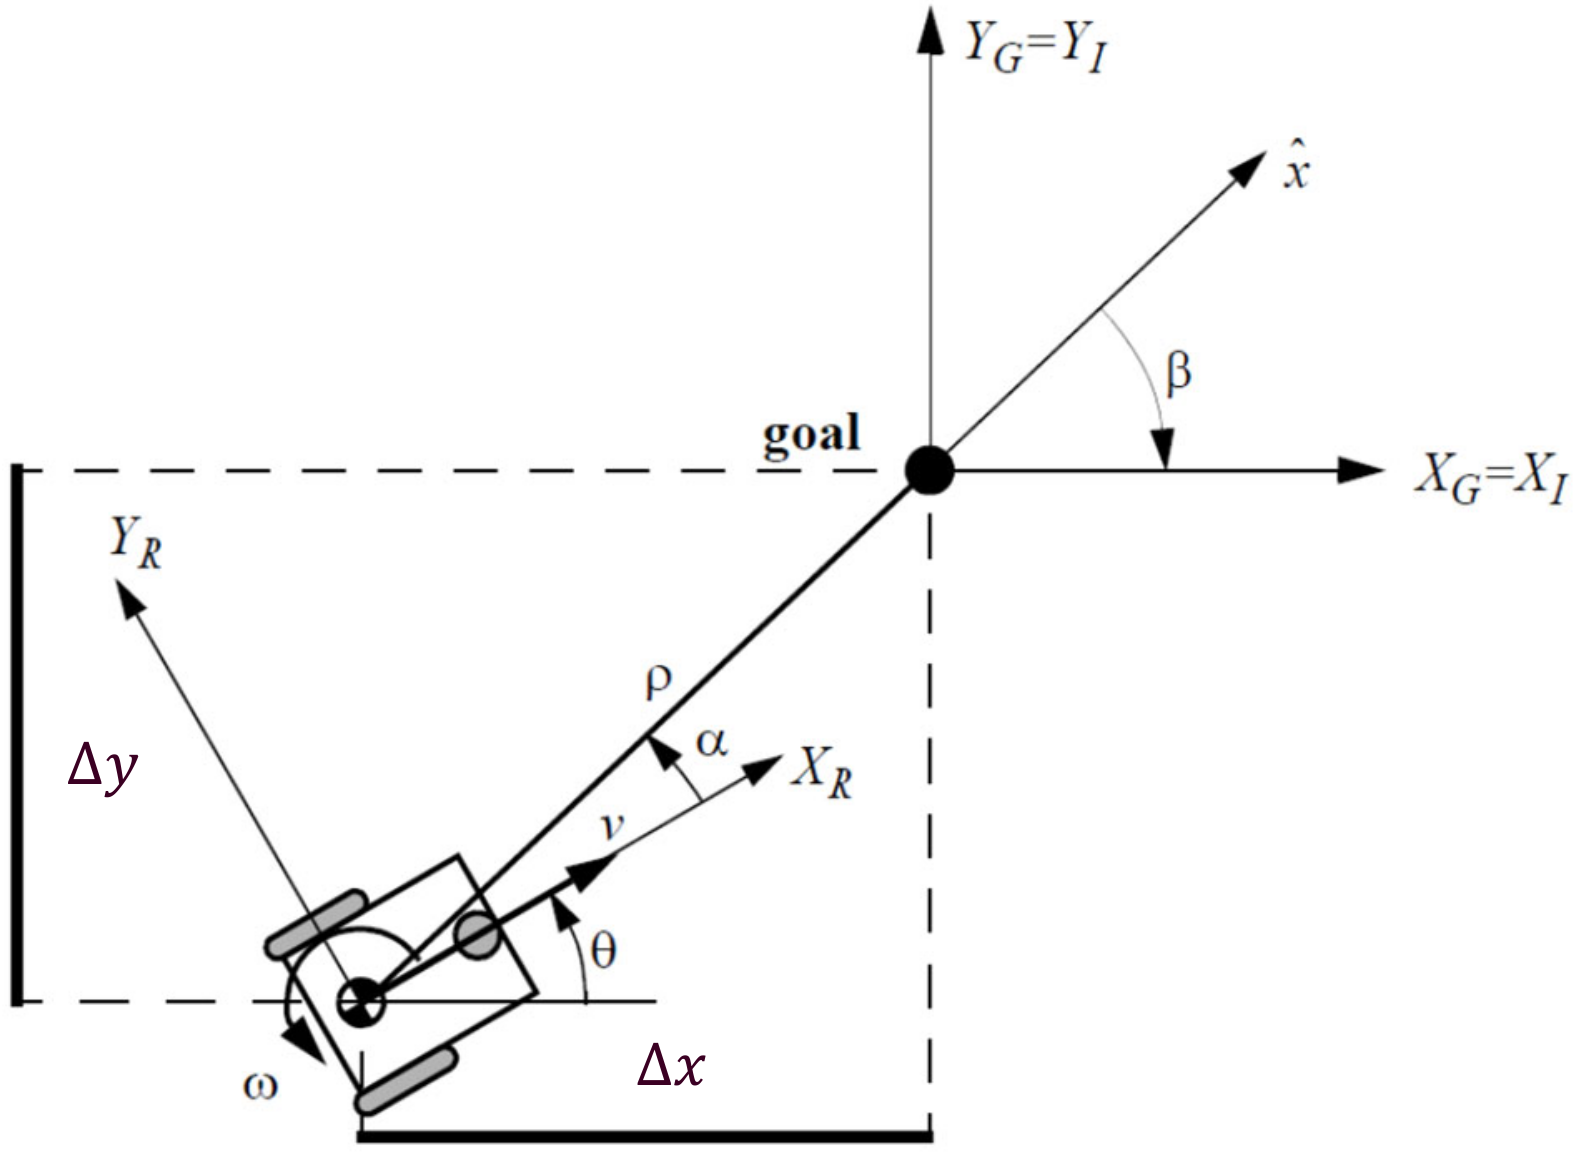
\includegraphics[width=\linewidth]{./Figures/03_MotionControl.png}
\begin{itemize}
    \item Drive robot from ${}_I[x, y, \delta]$ to ${}_I[0, 0, 0]$
    \ides{Error:} $e = [x, y, \delta]^\transpose$
    \item Get control inputs as $
        \begin{bmatrix}
            v(t)\\
            \omega(t)
        \end{bmatrix} = K \cdot e = K
        \begin{bmatrix}
            x\\
            y\\
            \theta
        \end{bmatrix}$
    \item Find $K$ such that $lim_{t \to \infty} e(t) = 0
        \begin{bmatrix}
            \dot x\\
            \dot y\\
            \dot \theta
        \end{bmatrix}_I =
        \begin{bmatrix}
            \cos \theta & 0\\
            \sin \theta & 0\\
            0 & 1
        \end{bmatrix}
        \begin{bmatrix}
            v\\
            \omega
        \end{bmatrix}$
    \item Polar Coordinate Transformation:
        \begin{itemize*}
            \item $\rho = \sqrt{\bigtriangleup x^2 + \bigtriangleup y ^2}$
            \item $\alpha = -\theta + \mathrm{atan2}(\bigtriangleup y, \bigtriangleup x)$
            \item $\beta = -\theta - \alpha$
            \item $\alpha, \beta \in [-\pi, \pi]$
        \end{itemize*}
    \item If $\alpha \in (-\frac{\pi}{2}, \frac{\pi}{2})$: $
        \begin{bmatrix}
            \dot \rho\\
            \dot \alpha\\
            \dot \beta
        \end{bmatrix} =
        \begin{bmatrix}
            -\cos \alpha & 0\\
            \frac{\sin \alpha}{\rho} & -1\\
            -\frac{\sin \alpha}{\rho} & 0
        \end{bmatrix}
        \begin{bmatrix}
            v\\
            \omega
        \end{bmatrix}$
    \item Otherwise: $
        \begin{bmatrix}
            \dot \rho\\
            \dot \alpha\\
            \dot \beta
        \end{bmatrix} =
        \begin{bmatrix}
            \cos \alpha & 0\\
            -\frac{\sin \alpha}{\rho} & 1\\
            \frac{\sin \alpha}{\rho} & 0
        \end{bmatrix}
        \begin{bmatrix}
            v\\
            \omega
        \end{bmatrix}$
    \item Control Law: $
        \begin{bmatrix}
            \dot \rho\\
            \dot \alpha\\
            \dot \beta
        \end{bmatrix} =
        \begin{bmatrix}
            -k_\rho \rho \cos(\alpha)\\
            k_\rho \sin(\alpha - k_\alpha \alpha - k_\beta \beta)\\
            -k_\rho \sin(\alpha)
        \end{bmatrix}$
    \item $v$ has a constant sign for one run
    \item Stable if $k_\rho > 0, k_\beta < 0, k_\alpha - k_\rho > 0$
\end{itemize}

%! TEX root = ./main.tex

\section{Perception}
\begin{itemize}
    \item Raw Data $\implies$ Features $\implies$ Objects $\implies$ Places/Situations
\end{itemize}

\subsection{Sensors}
\subsubsection{Types of Sensors}
\begin{itemize}
    \ides{Proprioceptive (PC):} Measure values internally to the system
    \ides{Exteroceptive (EC):} Acquire information about the robots environment
    \ides{Passive (P):} Measure ambient environmental energy
    \ides{Active (A):} Emit energy into the environment and measure the environments reaction to it
        \begin{itemize*}
            \ipro More accurate
            \icon May interfere
            \icon May affect the characteristic one wants to measure
        \end{itemize*}
    \ides{Encoders:}
        \begin{itemize*}
            \item Convert linear/angular motion of a shaft to digital
            \item For control of motor-driven joints
        \end{itemize*}
    \ides{Heading Sensors:}
        \begin{itemize*}
            \item Determine orientation and inclination w.r.t some reference
            \ides{Gyroscope:}
                \begin{itemize*}
                    \item Absolute measure for heading
                    \ides{Mechanical:} Fast spinning wheel
                    \ides{Optical:} Laser beam in fiber coil; Measure phase shift
                \end{itemize*}
        \end{itemize*}
    \ides{Range Sensors:}
        \begin{itemize*}
            \item Traveled distance $d$ of a sound or electromagnetic wave after a \textbf{time of flight} $t$
            \item $d=ct$
            \item Sound: $c = 0.3\,\mathrm m / \mathrm{ms}$
            \item Light: $c = 0.3\,\mathrm m / \mathrm{ns}$
        \end{itemize*}
    \ides{GPS:}
        \begin{itemize*}
            \item Satellites send their position and time to the device
            \item Device computes location based on ToF
            \item Time synchronisation and measurement is critical
            \ides{RTK:} Measure of carrier wave phase - up to centimeter-level accuracy
        \end{itemize*}
\end{itemize}

\subsubsection{Uncertainty Representation}
\begin{itemize}
    \ides{Systematic Error:}
        \begin{itemize*}
            \item Deterministic
            \item Can be modelled and calibrated
        \end{itemize*}
    \ides{Random Error:}
        \begin{itemize*}
            \item Cannot be predicted
            \item Described statistically
        \end{itemize*}
    \item Density function identifies for each possible $x$ of RV $X$ a probability $f(x)$
        \begin{itemize*}
            \item $\int_{-\infty}^\infty f(x) \rmd x = 1$
            \item $\mu = E[X] = \int_{-\infty}^\infty x f(x) \rmd x$
            \item $\sigma^2 = E[(X - E[X])^2]$
        \end{itemize*}
    \ides{Error Propagation Law}
        \begin{itemize*}
            \item Error propagation in system with $n$ inputs and $m$ outputs $f: \R^n \to \R^m$, $f: X_1, \dots X_n \mapsto f(X_1, \dots, X_n) = Y_j$
            \item Uncertainty of $X_i$ is known
            \item Mapping between input covariance $C_X$ and output covariance $C_Y$: $C_Y = F_X C_X F_X^\transpose$
            \item $F_X = \bigtriangledown f_X =
                \begin{bmatrix}
                    \frac{\partial f_1}{\partial X_1} & \dots & \frac{\partial f_1}{\partial X_n}\\
                    \vdots & \ddots & \vdots\\
                    \frac{\partial f_m}{\partial X_1} & \dots & \frac{\partial f_m}{\partial X_n}
                \end{bmatrix}$
            \ides{$\mathbf{C_{X/Y}}$:} Covariance of input uncertainties/propagated uncertainties of the output
        \end{itemize*}
\end{itemize}

\subsection{Computer Vision}

\subsubsection{Camera Model}
\begin{itemize}
    % \ides{Pinhole Model:}
    %     \begin{itemize*}
    %         \item Black box with single hole
    %         \item Beam of rays enter through the \textbf{Optical Center/Center of Projection C}
    %         \item Inverted image is projected onto the \textbf{Image Plane}
    %     \end{itemize*}
    % \ides{Converging Lens:}
    %     \begin{itemize*}
    %         \item Focuses multiple rays from the same point on the object to the same point on the image plane
    %         \item All rays parallel to the \textbf{optical axis} converge at the \textbf{focal point}
    %         \item Rays passing through the \textbf{optical center} are not diverged
    %     \end{itemize*}
    % \\ \begin{minipage}[b]{0.49\linewidth}
    %     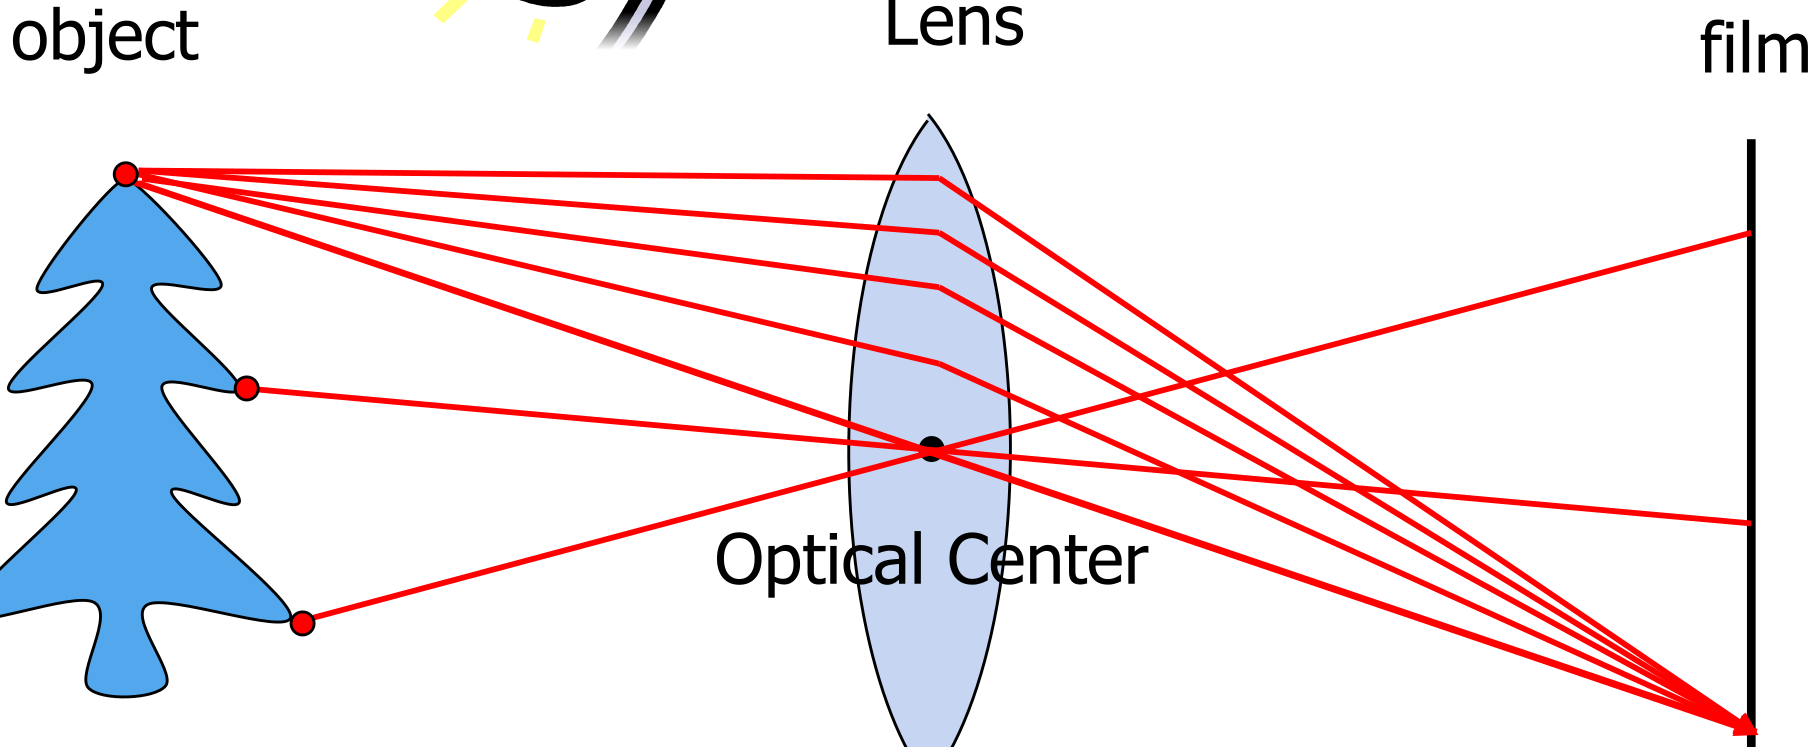
\includegraphics[width=\linewidth]{./Figures/04_Lens1.png}
    % \end{minipage}
    % \begin{minipage}[b]{0.49\linewidth}
    %     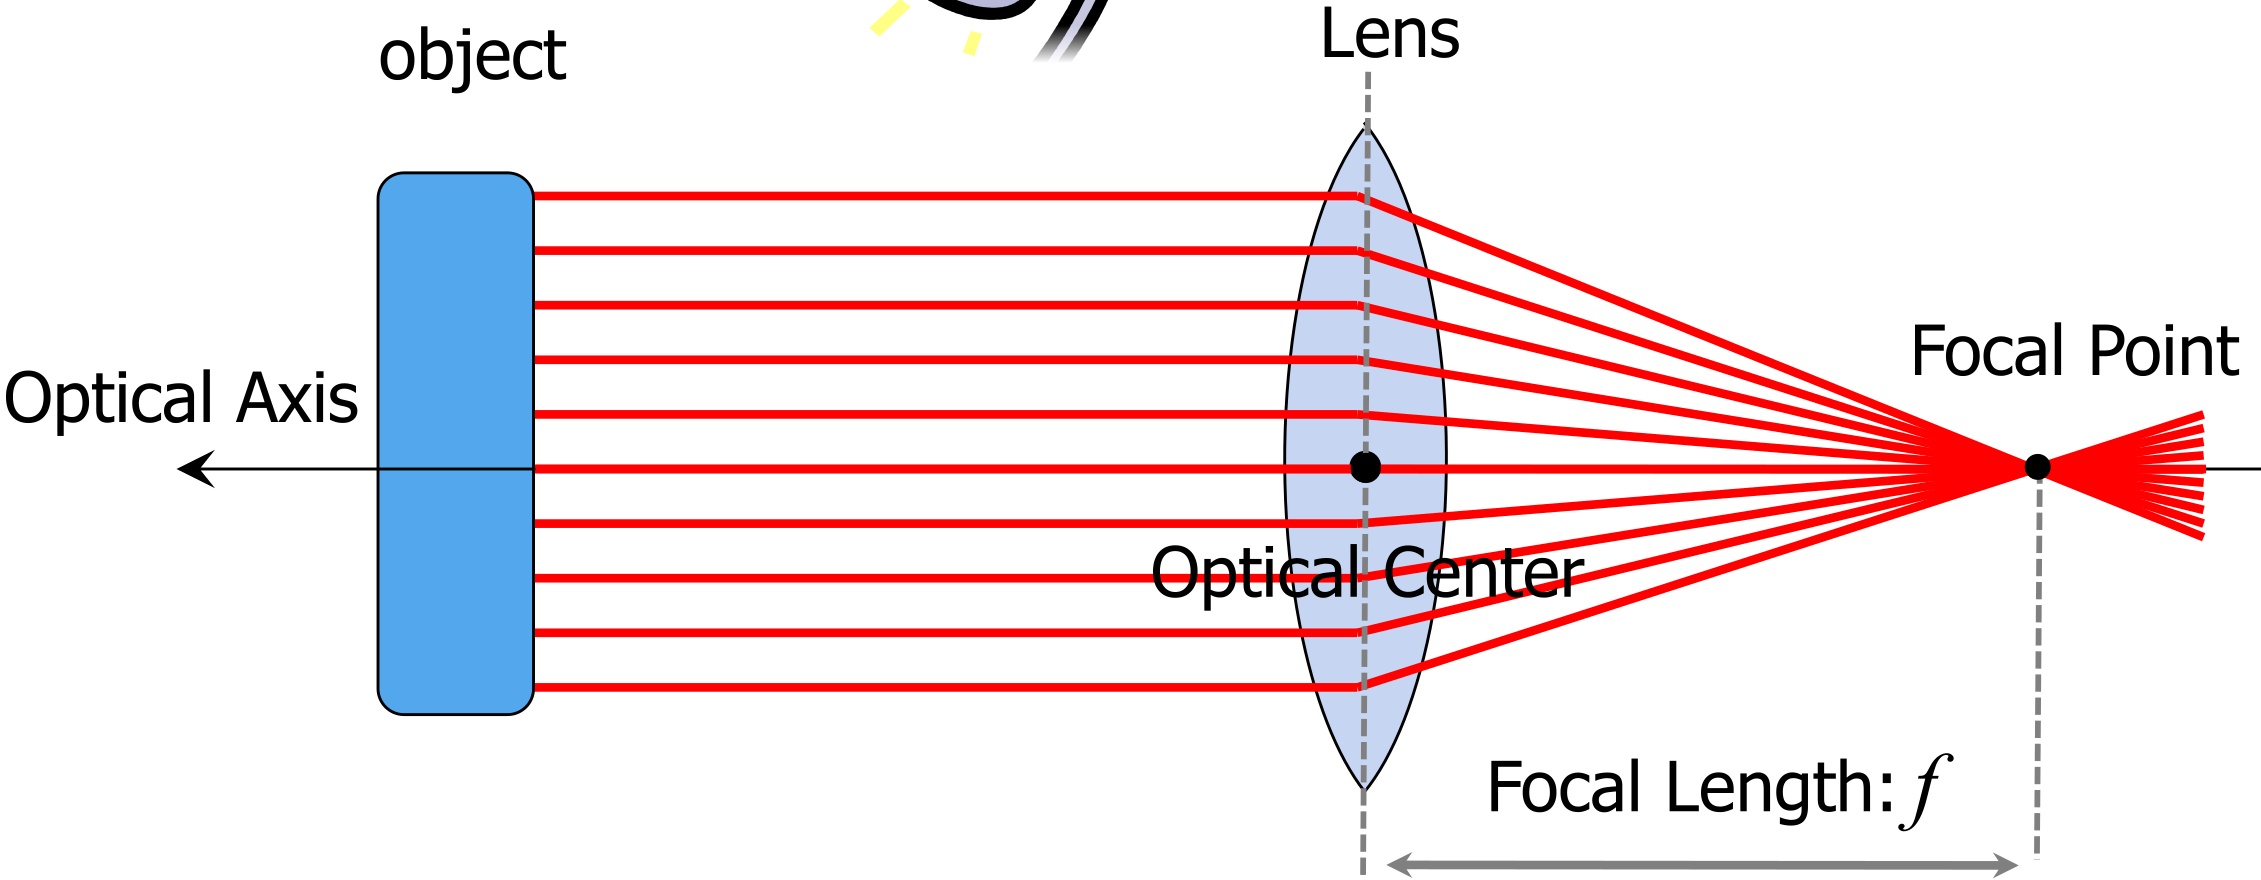
\includegraphics[width=\linewidth]{./Figures/04_Lens2.png}
    % \end{minipage}
    \ides{Thin Lens equation:} $\frac{1}{f} = \frac{1}{z} + \frac{1}{e}$
    \ides{Pinhole Approximation:} $z \gg f \implies f \approx e$
        \begin{itemize}
            \item I.e. lens is approximated as pinhole at distance $f$ from image plane
            \item If follows that $B' = \frac{f}{z}B$
        \end{itemize}
    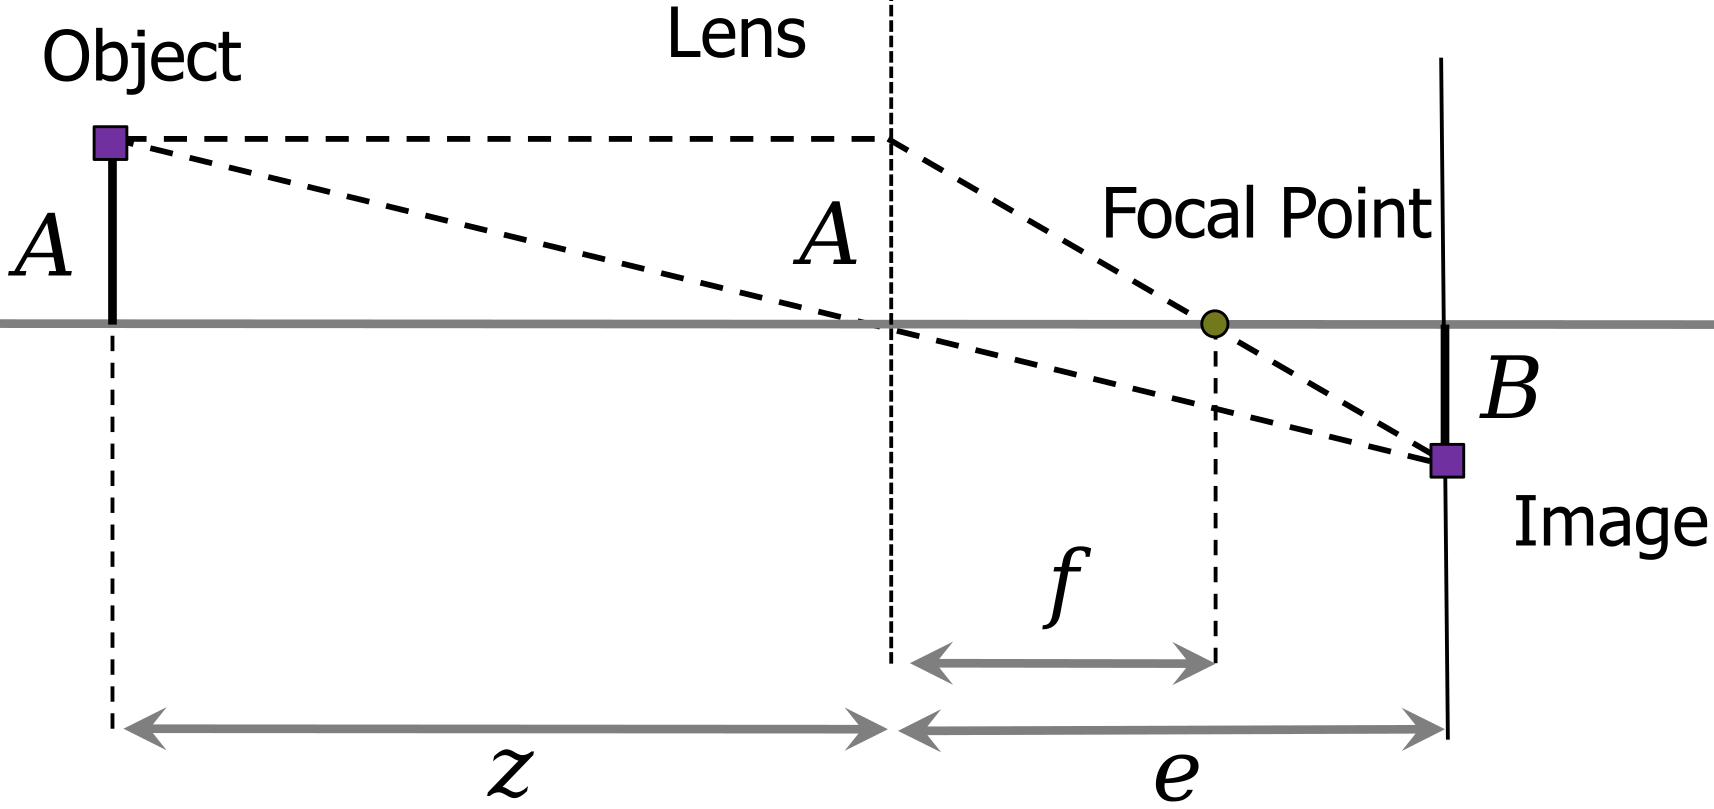
\includegraphics[width=\linewidth]{./Figures/04_ThinLensEquation.png}
\end{itemize}

\subsubsection{Perspective Camera}
\begin{itemize}
    % \item Image plane represented in front of $C$
    % \item Camera measures angles and not distances
    % \item Project pt $P_W = (x,y,z)$ onto $p_C = (u,v)$ on the image plane
    \ides{Perspective Equations:}\\
        \begin{itemize*}
            \item $x = f \frac{X_c}{Z_C}$
            \item $y = f \frac{Y_c}{Z_C}$
        \end{itemize*}\\
        \begin{itemize*}
            \item $u = u_0 + k x$
            \item $v = v_0 + k y$
            \ides{Scale factor $k$} $[\text{pixels}/\text{meter}]$
            \ides{Focal length in pixels:} $kf = \alpha$
        \end{itemize*}
        \begin{itemize}
            \item $\implies \tilde p =
                \begin{bmatrix}
                    \lambda u\\
                    \lambda v\\
                    \lambda
                \end{bmatrix} =
                \underbrace{
                \begin{bmatrix}
                    kf & 0 & u_0\\
                    0 & kf & v_0\\
                    0 & 0 & 1
                \end{bmatrix}}_{K}
                \begin{bmatrix}
                    X_C\\
                    Y_C\\
                    Z_C
                \end{bmatrix}$
        \end{itemize}
    \ides{Intrinsic Parameter $K$:} depending on camera
    \item Rigid Body transformation\\
        $\begin{bmatrix}
            X_C\\
            Y_C\\
            Z_C
        \end{bmatrix}=
        \underbrace{
        \begin{bmatrix}
            r_{11}  & r_{12} & r_{13}\\
            r_{21}  & r_{22} & r_{23}\\
            r_{31}  & r_{32} & r_{33}\\
        \end{bmatrix}}_{R}
        \begin{bmatrix}
        X_W\\
        Y_W\\
        Z_W
        \end{bmatrix} +
        \underbrace{
        \begin{bmatrix}
            t_1\\
            t_2\\
            t_3
        \end{bmatrix}}_{T} = [R \mid T]
        \begin{bmatrix}
            X_W\\
            Y_W\\
            Z_W\\
            1
        \end{bmatrix}$
\end{itemize}
\begin{minipage}[b]{0.49\linewidth}
    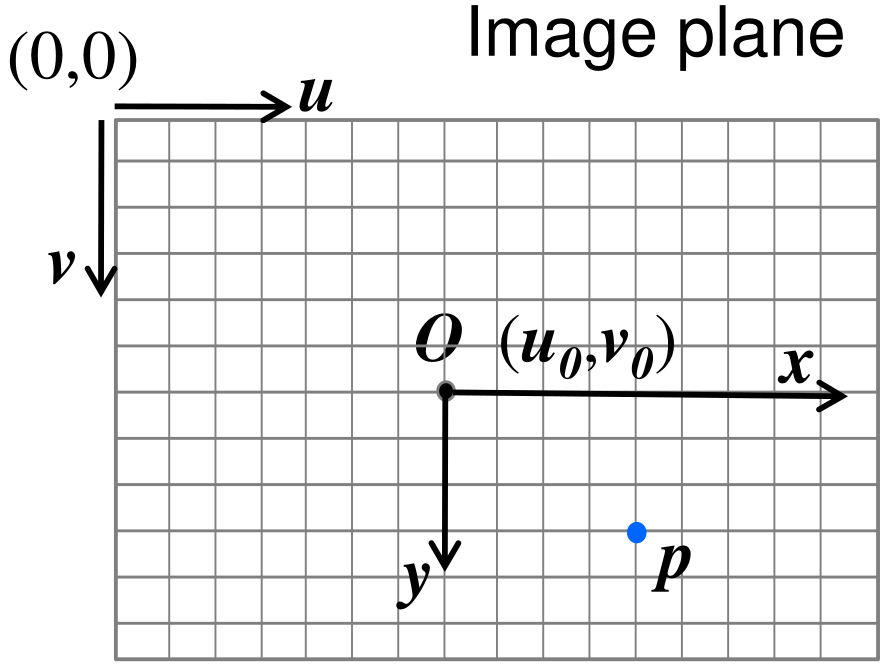
\includegraphics[width=\linewidth]{./Figures/04_PerspectiveProjection1.png}
\end{minipage}
\begin{minipage}[b]{0.49\linewidth}
    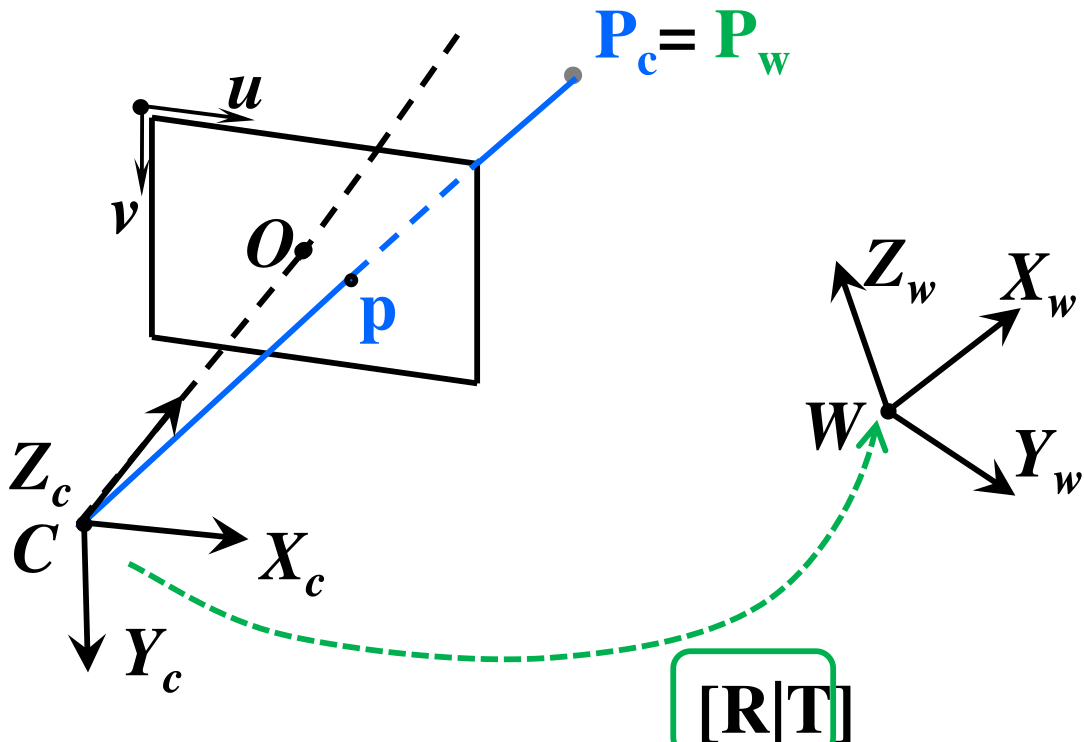
\includegraphics[width=\linewidth]{./Figures/04_PerspectiveProjection2.png}
\end{minipage}
\begin{itemize}
    \ides{Extrinsic Parameter $[R \mid T]$:} depending on transformation
    \ides{Perspective Projection:} $K[R \mid T]$
    \item $\implies \tilde p =
        \begin{bmatrix}
            \lambda u\\
            \lambda v\\
            \lambda
        \end{bmatrix} = K[R \mid T]
        \begin{bmatrix}
            X_W\\
            Y_W\\
            Z_W\\
            1
        \end{bmatrix}$
    \ides{Barrel Distortion}
        \begin{itemize}
            \item Straight lines get bent
            \ides{Barrel Distortion:} Image gets ``round''
            \ides{Pincushion Distortion:} Corners pulled out
            \item Model:
                $\begin{bmatrix}
                    u_d\\
                    v_d
                \end{bmatrix} = (1 + k_1 r^2)
                \begin{bmatrix}
                    u - u_0\\
                    v - v_0
                \end{bmatrix} +
                \begin{bmatrix}
                    u_0\\
                    v_0
                \end{bmatrix}$
                \begin{itemize}
                    \ides{Distortion Parameter $\mathbf{k_1}$:} Intrinsic parameter
                    \item $r^2 = (u - u_0)^2 + (v - v_0)^2$
                \end{itemize}
        \end{itemize}
\end{itemize}

\subsubsection{Omnidirectional Camera}
\begin{itemize}
    \ides{Dioptric:}
        \begin{itemize*}
            \item System of lenses
            \item $\sim 180^\circ$ FOV
        \end{itemize*}
    \ides{Catadioptric:}
        \begin{itemize*}
            \item Combination of lens and mirrors
            \item $> 180^\circ$ FOV
            \item Greatly distorted (can be removed depending on mirror)
        \end{itemize*}
        \begin{itemize}
            \ides{Central Camera:} Mirror shaped that all incoming rays have same \textit{single effective viewpoint}
                \begin{itemize}
                    \ides Correct mirror placement is important
                    \ipro Unwarping into perspective image possible
                    \ipro Can convert points in the image to spherical vectors
                    \ipro Can apply standard algorithms
                \end{itemize}
        \end{itemize}
    \ides{Polydioptric:}
        \begin{itemize*}
            \item Multiple cameras
            \item $\sim 360^\circ$ FOV
        \end{itemize*}
\end{itemize}

\subsubsection{Camera Calibration}
\begin{itemize*}
    \item Determine intrinsic (and extrinsic) camera parameters
    \item $\lambda
        \begin{bmatrix}
            u\\
            v\\
            1
        \end{bmatrix} = K [R|T]
        \begin{bmatrix}
            X_W\\
            Y_W\\
            Z_W\\
            1
        \end{bmatrix} \overset{!}{=} \linebreak
        \begin{bmatrix}
            m_{11} & \dots & m_{14}\\
            \vdots & \ddots & \vdots\\
            m_{31} & \dots & m_{34}
        \end{bmatrix}
        \begin{bmatrix}
            X_W\\
            Y_W\\
            Z_W\\
            1
        \end{bmatrix}$
    \item Find all $m_{ij}$
    \item Requires $\ge 6$ pts
    \item Done using least-square method
    \item Need to decompose the found matrix into $K, R, T$
    \item QR factorize $3 \times 3$ submatrix $m_{11}:m_{33} \Rightarrow K := R, R := R$
    \item Calculate $T = K^{-1}[m_14, m_{24}, m_{34}]^\transpose$
\end{itemize*}

\subsubsection{Stereo Vision}
\begin{minipage}[b]{0.49\linewidth}
    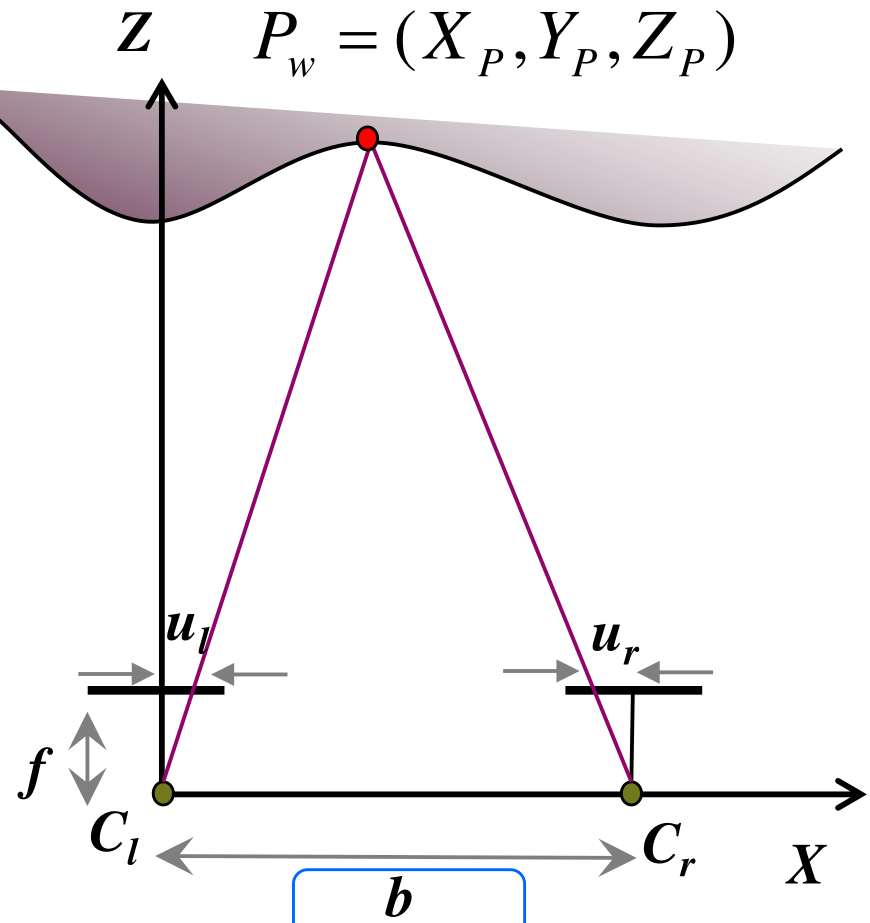
\includegraphics[width=\linewidth]{./Figures/04_StereoVision.png}
\end{minipage}
\begin{minipage}[b]{0.49\linewidth}
    \raggedright
    \begin{itemize}
        \item Obtain depth information from two cameras with known relative position
        \item Cameras need to be calibrated
        \item Calculating depth $Z_P$ of point $P_W$ (distance to $P_W$)
        \ides{Baseline $\mathbf{b}$:} Distance between the two cameras
    \end{itemize}
\end{minipage}
\begin{itemize}
    \ides{Disparity:} Difference in image location of the projection of a 3D point on the two image panes: $u_l - u_r$
    \item Two identical cameras aligned on $x$
        \begin{itemize}
            \item $Z_P = \frac{bf}{u_l - u_r}$
        \end{itemize}
    \item Two identical cameras in different Coordinate Systems
        \begin{itemize}
            \item $C_r$ is a rigid body transformation of $C_l$\\
            \item Triangulation
            \begin{itemize*}
                \item $\tilde p_l = \lambda_l
                    \begin{bmatrix}
                        u_l\\
                        v_l\\
                        1
                    \end{bmatrix} = K_l
                    \begin{bmatrix}
                        X_W\\
                        Y_W\\
                        Z_W
                    \end{bmatrix}$
                \item $\tilde p_r = \lambda_r
                    \begin{bmatrix}
                        u_r\\
                        v_r\\
                        1
                    \end{bmatrix} = K_r R
                    \begin{bmatrix}
                        X_W\\
                        Y_W\\
                        Z_W
                    \end{bmatrix} + T$
            \end{itemize*}
        \end{itemize}
    \ides{Disparity Map}
        \begin{itemize}
            \item Compute disparity for corresponding points of every pixel
            \item Can compute the depth from it and reconstruct 3D scene
        \end{itemize}
\end{itemize}

\subsubsection{Correspondence Search}
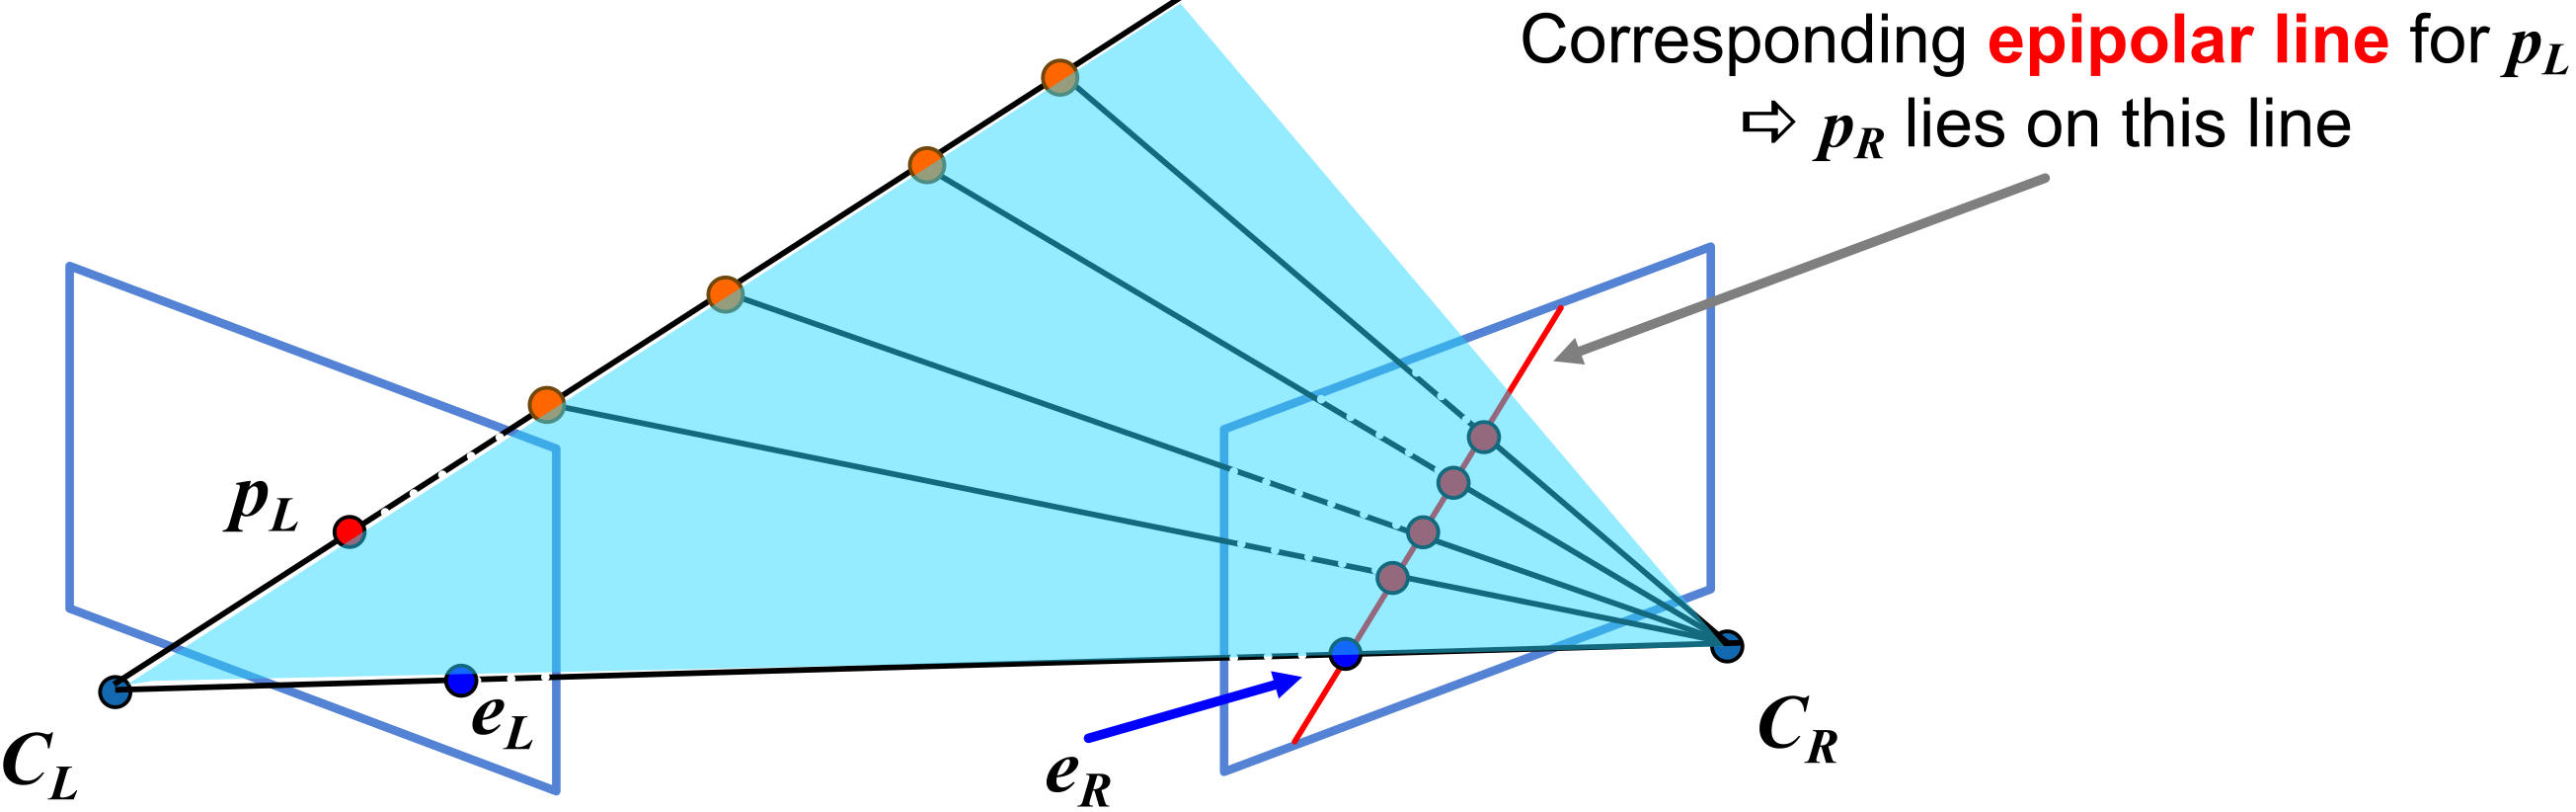
\includegraphics[width=\linewidth]{./Figures/04_EpopolarPlan.png}
\begin{itemize}
    \item Identify corresponding points in two images of the same scene
    \item Measure similarity of two pts using a similarity measurement
    \ides{Epipolar Plane:} Spanned by $C_l$, $C_r$ and some pt $P_W$
    \ides{Epipolar Line:} Projection of the ray from one camera through points in the other camera
    \ides{Epipole:} Projection of other camera in image plane
        \begin{itemize*}
            \item All epipolar lines go through it
        \end{itemize*}
    \ides{Epipolar Constraint:} Correspond of pt of left images lies on the epipolar line of the right image
    \ides{Epipolar Rectification:} Transform both images to make epipolar lines collinear and parallel:
        \begin{itemize*}
            \item[1)] Remove radial distortion
            \item[2)] \textbf{Warping:} Reprojection of both images to same plane
        \end{itemize*}
\end{itemize}

\subsubsection{Triangulation}
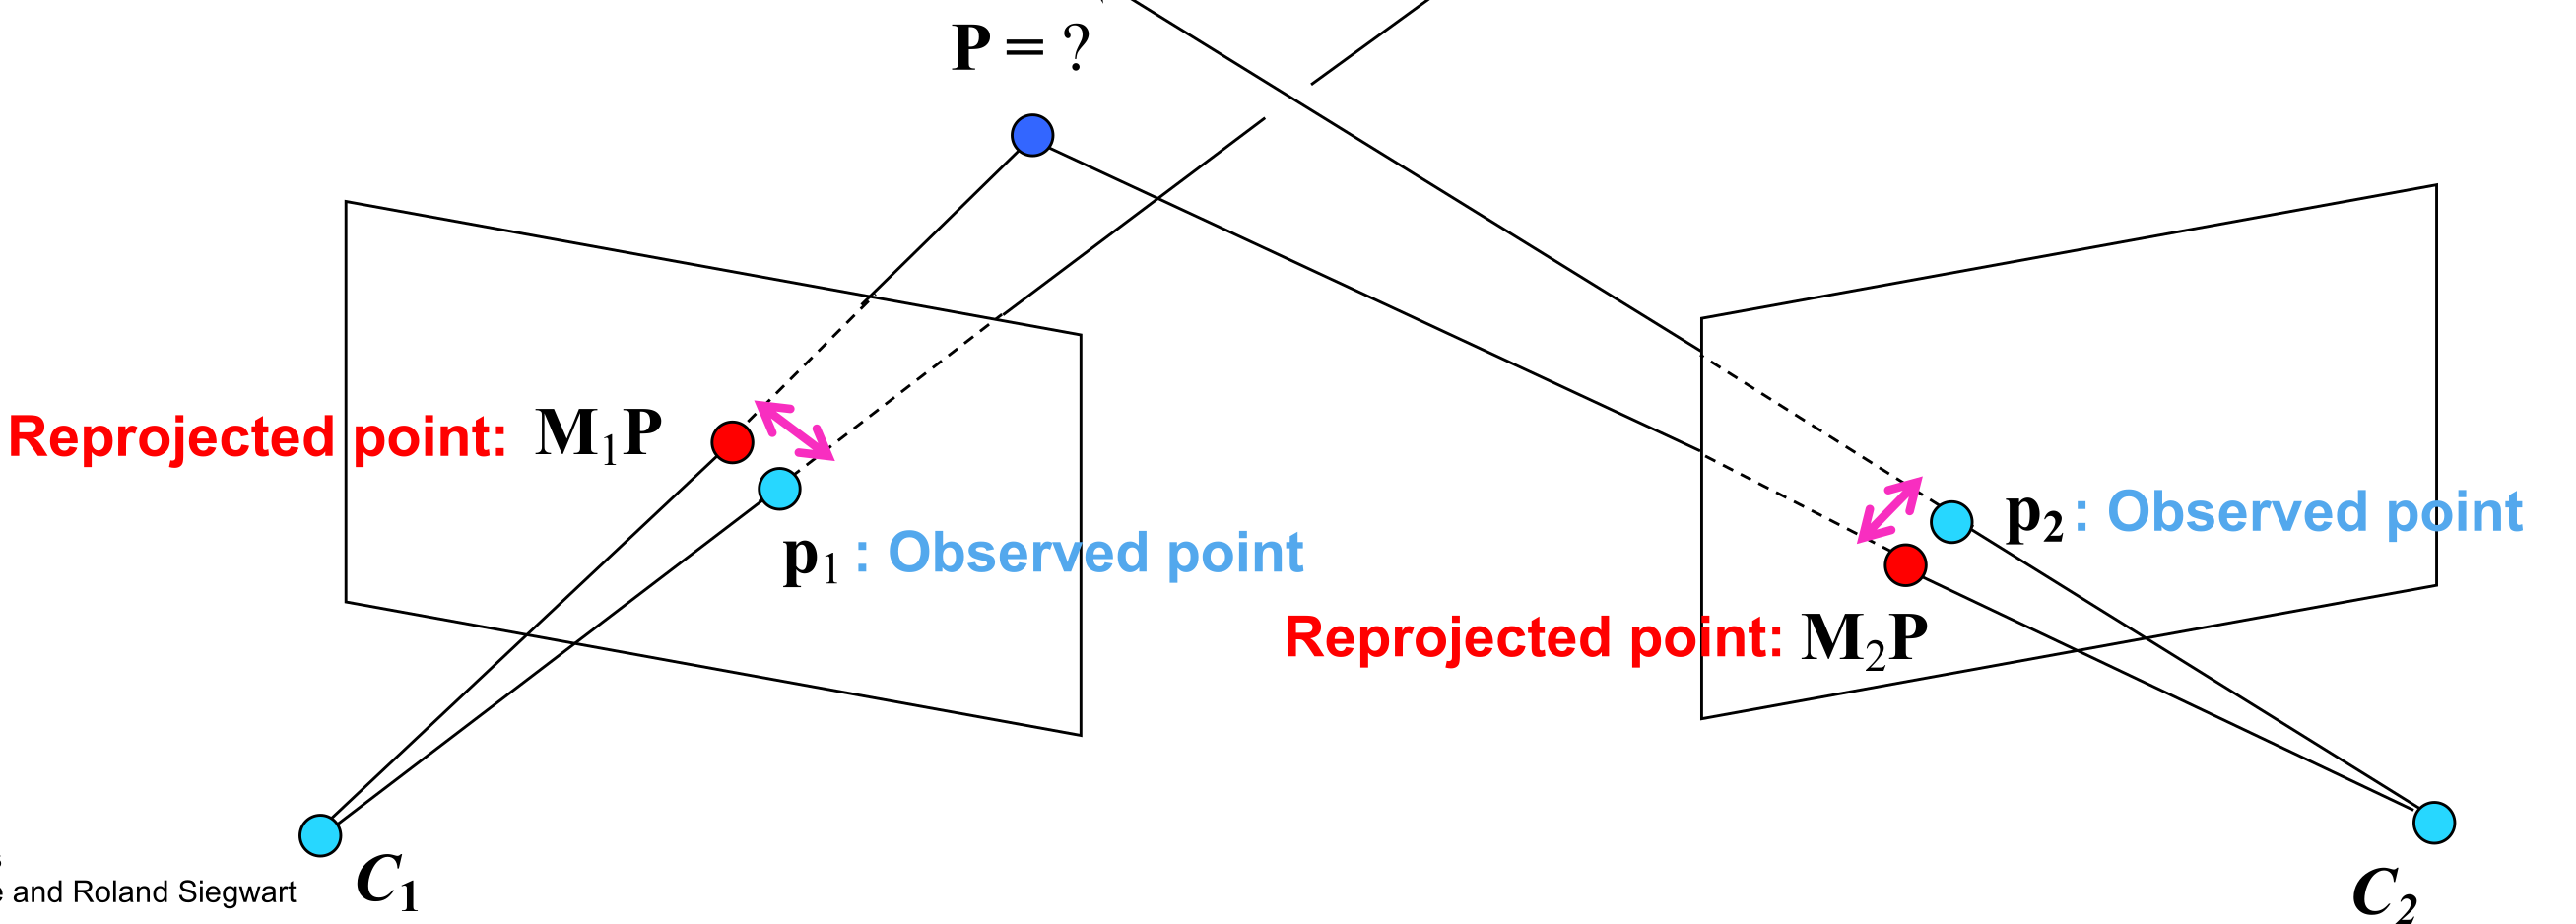
\includegraphics[width=\linewidth]{./Figures/04_Triangulation.png}
\begin{itemize}
    \item Find 3D coordinate of a point given the projections on multiple image planes
    \item $R_i, T_i, K_i$ are known
    \item
        \begin{itemize*}
            \item $\lambda_1
                \underbrace{\begin{bmatrix}
                    u_1\\
                    v_1\\
                    1
            \end{bmatrix}}_{p_1} = \underbrace{K_1[I \mid 0]}_{M_1}
                \underbrace{\begin{bmatrix}
                    X_x\\
                    Y_w\\
                    Z_w\\
                    1
                \end{bmatrix}}_{P}$
            \item $\lambda_2
                \begin{bmatrix}
                    u_2\\
                    v_2\\
                    1
                \end{bmatrix} = K_2[R \mid T]
                \begin{bmatrix}
                    X_x\\
                    Y_w\\
                    Z_w\\
                    1
                \end{bmatrix}$
        \end{itemize*}
    \item No unique solution due to noise and errors
    \ides{Linear Approach:} Solved using SVD
    \ides{Reprojection Approach:} Minimize Sum of Square Reprojection Error $\mathrm{SSRE} = \norm{P_1 - M_1 P}^2 + \norm{p_2 - M_2 P}^2$
    \item Baseline is important:
        \begin{itemize}
            \ides{Too Small:} Large depth error
            \ides{Too Large:}
                \begin{itemize*}
                    \item Objects may be visible only from one camera
                    \item Difficult search problem for close objects
                \end{itemize*}
        \end{itemize}
\end{itemize}

\subsubsection{Structure from Motion (SfM)}
\begin{itemize}
    \item Given corresponding image points $\{(u_1^i, v_1^i), (u_2^i, v_2^i)\}$, recover:
        \begin{itemize*}
            \item 3D location $P_i$ of all $n$ pts
            \item Relative pose of right camera $R, T$
            \item Camera intrinsic $K$ (optionally)
        \end{itemize*}
    \item Assume $K$ is known
    \ides{Knowns:} $4n$: $n$ correspondences
    \ides{Unknowns:} $5 + 3n$: rotation ($3$), translation ($2$, since scale cannot be recovered), $n$ 3D pts ($3n$)
    \item Solution exists iff $4n \ge 5 + 3n \implies n \ge 5$
    \ides{Crossp.:} $a \times b =
        \begin{bmatrix}
            0 & -a_z & a_y\\
            a_z & 0 & -a_x\\
            -a_y & a_x & 0
        \end{bmatrix}
        \begin{bmatrix}
            b_x\\
            b_y\\
            b_z
        \end{bmatrix} = [a]_\times b$
    \ides{Epipolar Constraint:} $p_2^T E p_1 = 0$
    \ides{Essential Matrix:} $E = [T]_\times R$
        \begin{itemize}
            \item Computed with $\ge 5$ correspondences
            \item Can be decomposed into $R$ and $T$
        \end{itemize}
    \ides{Normalized Img Coordinates:} $p = [\bar u, \bar v, 1]^\transpose = K^{-1}[u, v, 1]^\transpose$
    \ides{8-pt Algorithm}
        \begin{itemize*}
            \item Algorithm to compute essential matrix
            \item Uses $\ge 8$ pts
        \end{itemize*}
        \begin{itemize}
            \item $p_2^\transpose E p_1 = [\bar u_2, \bar v_2, 1]
                \begin{bmatrix}
                    e_11 & e_12 & e_13\\
                    e_21 & e_22 & e_23\\
                    e_31 & e_32 & e_33
                \end{bmatrix}
                \begin{bmatrix}
                    \bar u_1\\
                    \bar v_1\\
                    1
                \end{bmatrix} = 0$
            \item $\underbrace{[u_2u_1, u_2v_1, u_2, v_2u_1, v_2v_1, v_2, u_1, v_1, 1]}_{Q: \text{known}} \cdot \linebreak \underbrace{[e_{11}, e_{12}, \dots, e_{33}]}_{\text{unknown}} = 0$
            \item For $8$ non-coplanar pts, unique solution is given by the EV of $Q$ corresponding to the smallest Eigenvalue
        \end{itemize}
\end{itemize}

\subsubsection{Image Filtering}
\begin{itemize}
    \ides{Linear:} Replace each pixel by a linear combination of its neighbours
    \ides{Shift-Invariant:} Same operation is performed on every point on the image
    \ides{Filter $\mathbf{H}$:} aka. \textit{kernel, mask, window}
    \ides{Boundaries:} Need to handle specially:
        \begin{itemize*}
            \item Ignore
            \item Zero padding
            \item Pad with edge value
            \item Mirror boundary
            \item Wrap around from other side
        \end{itemize*}
    \ides{Normalization:} Prevent img from getting brighter/darker
    \ides{Correlation:} $J(x) = F \circ I(x,y) = \sum_{i=-N}^N \sum_{j=-M}^M F(i,j) I(x + i, y + j)$
        \begin{itemize}
            \item Not associative
        \end{itemize}
    \ides{Convolution:} $J(x) = F \ast I(x,y) = \sum_{i=-N}^N \sum_{j=-M}^M F(i,j) I(x - i, y - j)$
        \begin{itemize}
            \item Equivalent to correlation except that the filter is flipped before correlating
            \item Same result to correlation if the filter is symmetric
            \item Is associative: $F \ast (G \ast I) = (F \ast G) \ast I$
        \end{itemize}
    \ides{Correlation Cost: (per pixel)}
        \begin{itemize}
            \ides{2D:}
                \begin{itemize*}
                    \ides{Mult.:} $(2N + 1)^2$
                    \ides{Add.:} $(2N - 1)^2 - 1$
                \end{itemize*}
            \ides{$\mathbf{2 \times 1D}$:}
                \begin{itemize*}
                    \ides{Mult.:} $2(2N + 1)$
                    \ides{Add.:} $4N$
                \end{itemize*}
            \ides{$\mathbf{2 \times 1D}$ with const.:}
                \begin{itemize*}
                    \ides{Mult.:} $1$
                    \ides{Add.:} $4N$
                \end{itemize*}
        \end{itemize}
    \ides{Derivation:} $J(x) = \frac{I(x+1)-I(x-1)}{2}$
    \ides{Smoothing:}
        \begin{itemize}
            \item For blurring or noise detection
            \ides{1D Gaussian:} $G_\sigma(x) = \frac{1}{\sigma \sqrt{2 \pi}} \mathrm e^{-\frac{x^2}{2 \sigma^2}}$
            \ides{2D Gaussian:} $G_\sigma(x, y) = \frac{1}{2 \pi \sigma^2} \mathrm e^{-\frac{x^2 + y^2}{2 \sigma ^2}} = g_\sigma(x) \cdot g_\sigma(y) =
                \tfrac{1}{\sigma \sqrt{2\pi}} \mathrm e^{\frac{-x^2}{2\sigma^2}}
                \cdot
                \tfrac{1}{\sigma \sqrt{2\pi}} \mathrm e^{\frac{-y^2}{2\sigma^2}}$
                \begin{itemize}
                    \item Is separable
                \end{itemize}
        \end{itemize}
    \ides{Similarity Measure}
        \begin{itemize}
            \ides{Sum of Square Diff.:} $\mathrm{SSD}(x) =
                \sum_i (F(i) - I(x+i))^2 =
                \sum_i F(i)^2 + \sum_i I(x+i)^2 - 2 \sum_i (F(i) I(x+i))$
            \ides{Normalized Cross Correlation:} $\mathrm{NCC} =
                \frac{\sum_i (F(i)I(x + i))}
                {\sqrt{\sum_i F(i)^2} \sqrt{\sum_i I(x+i)^2}}$
            \ides{Zero-Mean Normalized Cross Correlation (ZNCC)}: Invariant to local average intensity. Maximize: $\mathrm{ZNCC}(x) =
                \frac{\sum_i (F(i)- \mu_F)(I(x + i) - \mu_{I_x})}
                {
                    \sqrt{\sum_i (F(i) - \mu_F)^2}
                    \sqrt{\sum_i (I(x+i) - \mu_{I_x})^2}
                }$
                \begin{itemize*}
                    \item $\mu_F = \frac{\sum_i F(i)}{2N + 1}$
                    \item $\mu_{I_x} = \frac{\sum_i I(x+i)}{2N + 1}$
                \end{itemize*}
        \end{itemize}
    \ides{Template Matching:} Use template as filter and apply similarity measure
    \ides{Edge Detection:}
        \begin{itemize*}
            \item[1)] Noise reduction
            \item[2)] Gradient $S^\prime = (G_\sigma \ast I)^\prime = G_\sigma^\prime \ast I$
            \item[3)] Thresholding
            \item[4)] Non-maximal suppression
        \end{itemize*}
        \begin{itemize}
            \ides{Derivation of Gaussian:} $G_\sigma^\prime(x, y) = \frac{\partial G_\sigma(x, y)}{\partial x} + \frac{\partial G_\sigma(x, y)}{\partial y}$
                \begin{itemize*}
                    \item Edges at min/max
                \end{itemize*}
            \ides{Laplacian of Gaussian:} $\mathrm{LoG} = G_\sigma^{\prime\prime}(x, y) = \frac{\partial^2 G_\sigma(x, y)}{\partial x^2} + \frac{\partial^2 G_\sigma(x, y)}{\partial y^2}$
                \begin{itemize*}
                    \item Edges at zero crossing
                \end{itemize*}
            \ides{Prewitt:}
                \\ \begin{itemize*}
                    \item $F_x = \left[
                        \begin{array}{c | c | c}
                            -1 & 0 & 1\\
                            -1 & 0 & 1\\
                            -1 & 0 & 1
                    \end{array} \right]$
                    \item $F_x = \left[
                        \begin{array}{c | c | c}
                            1 & 1 & 1\\
                            0 & 0 & 0\\
                            -1 & -1 & -1
                    \end{array} \right]$
                \end{itemize*}
            \ides{Sobel:}
                \\ \begin{itemize*}
                    \item $F_x = \left[
                        \begin{array}{c | c | c}
                            -1 & 0 & 1\\
                            -2 & 0 & 2\\
                            -1 & 0 & 1
                    \end{array} \right]$
                    \item $F_x = \left[
                        \begin{array}{c | c | c}
                            1 & 2 & 1\\
                            0 & 0 & 0\\
                            -1 & -2 & -1
                    \end{array} \right]$
                \end{itemize*}
            \ides{Roberts:}
                \begin{itemize*}
                    \item $F_x = \left[
                        \begin{array}{c | c}
                            0 & 1\\
                            1 & 0\\
                    \end{array} \right]$
                    \item $F_x = \left[
                        \begin{array}{c | c}
                            1 & 0\\
                            0 & 1\\
                    \end{array} \right]$
                \end{itemize*}
        \end{itemize}
\end{itemize}

\subsubsection{Point Features}
\begin{itemize}
    \ides{Harris Corner Detection:} Patch at $(x,y)$ of size $P$ has great difference to all surrounding patches $(x + \Delta x, y + \Delta y)$
        \begin{itemize}
            \item $\mathrm{SSD}(\Delta x, \Delta y) = \sum_{x,y \in P}(I(x,y) - I(x + \Delta x, y + \Delta y))^2$
            \item $\Rightarrow \mathrm{SSD}(\Delta x, \Delta y) \approx \sum_{x,y \in P}(I_x(x,y)x - I_y(x, y)y)^2$
                \\ \begin{itemize*}
                    \item $I_{x} = \frac{\partial I(x,y)}{\partial x}$
                    \item $I_{y} = \frac{\partial I(x,y)}{\partial y}$
                    \item Using first-order Taylor approx
                \end{itemize*}
            \item $\Rightarrow \mathrm{SSD}(\Delta x, \Delta y) \approx [\Delta x, \Delta y]M[\Delta x, \Delta y]^\transpose$
                \\ \begin{itemize*}
                    \item $M = \sum_{x,y \in P}
\begin{bmatrix}
    I_x^2 & I_xI_y\\
    I_xI_y & I_y^2
\end{bmatrix}
\allowbreak = R^{-1}
\begin{bmatrix}
    \lambda_1 & 0\\
    0 & \lambda_2
\end{bmatrix} R$
                \end{itemize*}
            \item \begin{itemize*}
                \ides{$\mathbf{\lambda_1, \lambda_2}$ small:} Flat region
                \ides{$\mathbf{\lambda_1 >> \lambda_2}$:} Edge
                \ides{$\mathbf{\lambda_1 << \lambda_2}$:} Edge
                \ides{$\mathbf{\lambda_1, \lambda_2}$ large:} Corner
            \end{itemize*}
            \ides{Cornerness Function:} $C = \text{det} - \kappa \ \text{trace}^2(M)$
                \\ \begin{itemize*}
                    \item Extract local minima
                    \item Used since calculating eigenvalues is expensive
                    \item $\kappa$ is magic number
                \end{itemize*}
            \ides{Invariant to:}
                \begin{itemize*}
                    \item Rotation
                    \item Linear intensity change
                \end{itemize*}
            \ides{Not invariant to:} Scale change
        \end{itemize}
    \ides{Scale Invariant Feature Transform (SIFT) Features:}
        \begin{itemize}
            \item Detect blobs
            \item Assigns each keypoint a orientation and descriptor
            \ides{Keypoint Detection:}
                \begin{itemize*}
                    \item[1)] Downscale image multiple times
                    \item[2)] Gaussian blur each at different rates
                    \item[3)] Calculate \textit{Difference of Gaussian (DoG)} (subtract successive smoothed images)
                    \item[4)] Find keypoints (local extrema in the DoG)
                \end{itemize*}
            \ides{Keypoint Orientation:}
                \begin{itemize*}
                    \item[1)] Generate gradient orientation histogram for each keypoint
                    \item[2)] Orientation is value of highest peak in histogram
                \end{itemize*}
            \ides{Keypoint Descriptor:}
                \begin{itemize*}
                    \item[1)] Divide neighbourhood into $4 \times 4$ regions
                    \item[2)] Compute orientation histograms along $8$ orientations
                    \item[3)] Concatenate $4 \times 4 \times 8 = 128$ values in vector
                \end{itemize*}
            \ipro High robustness
            \ipro Invariant to rotation
        \end{itemize}
    \ides{Features from Accelerated Segment Test (FAST) Detector:}
        \begin{itemize*}
            \item Detects corners
            \item Look at $16$ pixels around target pixel
            \item If they are all significantly darker/brighter, we have a FAST corner
            \ipro Fast
            \icon Not robust against noise
        \end{itemize*}
    \ides{Binary Robust Independent Elementary Features (BRIEF) Descriptor:}
        \begin{itemize}
            \item Detect blobs
                \begin{itemize*}
                    \item[1)] ``Random'' (predefined) selection of pixel pairs
                    \item[2)] Compare intensity of pairs and store result in descriptor
                    \item[3)] Matching done with Hamming Distance
                \end{itemize*}
            \ipro High speed in description and matching
            \icon Not scale invariant
            \icon Not rotation invariant
        \end{itemize}
    \ides{Binary Robust Invariant Scalable Keypoints (BRISK) Detector}
        \begin{itemize*}
            \item Detect blobs
            \item[1)] Detect corners using FAST
            \item[2)] Compare intensity similar to BRIEF but in some specific geometric pattern
            \ipro High speed
            \ipro Rotation and scale invariant
            \icon Slower than BRIEF
        \end{itemize*}
\end{itemize}

\subsubsection{Place Recognition}
\begin{itemize}
    \item Training set of images needed to create structure
    \ides{Bag of features:} Bag of descriptors of a word
        \begin{itemize*}
            \item Image is described by this set
            \item Sectional information is removed
        \end{itemize*}
    \ides{Visual Word:} Single number representing a high-dimensional descriptor
        \begin{itemize*}
            \item Done by \textbf{k-means clustering}
            \item Bag of features $\Rightarrow$ bag of visual words
        \end{itemize*}
    \ides{Visual Vocabulary:} DB of visual words created by many training images
    \item Scene is collection of visual words
    \item Efficiently find matches:
        \begin{itemize}
            \ides{Vocabulary Tree:} Hierarchical arrangement of visual vocabulary (I guess)
                \begin{itemize*}
                    \item Leaf holds image which matches the feature
                    \item By feeding in features of new images, we get a bag of matching images
                    \item Number of matches determines the probability
                \end{itemize*}
            \ides{Inverted File DB:}
                \begin{itemize*}
                    \item List of all possible visual words points to list containing all images containing this feature
                    \item Query DB for all features of a given list and count occurrences of a certain image (using voting array)
                \end{itemize*}
        \end{itemize}
    \ides{Term Frequency-Inverse Document Frequency (tf-idf):} Not all words are equally important
        \begin{itemize}
            \item Measure importance of visual word inside image
            \item Used for voting array
            \item For word $w_i$ in img $j$:
                \begin{itemize*}
                    \item $\text{tf-ids}_{ij} = \mathrm{tf}_{ij} \cdot \mathrm{idf}_i$
                    \item $\mathrm{tf}_{ij} = \frac{\# \text{occur. of } w_i \text{in } j}{\# \text{words in } j}$
                    \item $\mathrm{idf}_{i} = \log \frac{|\text{Img}|}{|\{\text{img} \mid w_i \in \text{img}\}|}$
                \end{itemize*}
        \end{itemize}
    \ides{FABMAP}
        \begin{itemize*}
            \item Place recognition
            \item Assume: worlds is set of discrete places
            \ides{Place:} vector of visual words at that scene
            \item Calculate probability of being at a know location
            \item Frequent occurring objects are suppressed
            \ipro High performance
        \end{itemize*}
\end{itemize}

\subsubsection{Line Extraction}
\begin{itemize}
    \ides{Task:} Given set of pts, find best fitting line
        \begin{itemize*}
            \item Do not have to figure out which pts belong to which line
        \end{itemize*}
    \ides{Split-and-Merge:}
        \begin{itemize}
            \item[1)] \textbf{Split:}
                \begin{itemize*}
                    \item[a)] Fit line through point set (or take end-pts)
                    \item[b)] Find most distant pt
                    \item[c)] If distance $>$ threshold, split set and repeat
                \end{itemize*}
            \item[2)] \textbf{Merge:} If two consecutive line segments are almost collinear, merge them
            \icon Sensitive to outliers
        \end{itemize}
    \ides{Random Sample Consensus (RANSAC):}
        \begin{itemize*}
            \item[1)] Draw line through two randomly selected pts
            \item[2)] Compute distance of all pts to it
            \item[4)] Repeat $k = \frac{\log({1 - p)}}{\log(1 - w^2)}$ times
                \begin{itemize*}
                    \ides{w:} fraction of inliers
                    \ides{p:} prob of finding set of pts free of outliers
                \end{itemize*}
            \item[5)] Select line with least total error
        \end{itemize*}
        \begin{itemize}
            \icon Non-Deterministic
        \end{itemize}
    \ides{Hough-Transform:}
        \begin{itemize}
            \item Each pt in image space defines a sinusoid in Hough space
        \end{itemize}
        \begin{itemize*}
            \item[1)] For each pt compute $\rho = x \cos \theta + y \sin \theta, \theta \in [0, 180]$
            \item[2)] Capture votes for parameters
            \item[3)] Find $(rho, \theta)$ with most votes
        \end{itemize*}
\end{itemize}

%! TEX root = ./main.tex

\section{Localization}
\begin{itemize}
    \item Problems:
        \begin{itemize}
            \ides{Position tracking:} Keep track of known location
            \ides{Global localization:} Localize without initial location
            \ides{Kidnapping robot problem:} Robot is moved to new location
        \end{itemize}
    \ides{Map Representation}
        \begin{itemize}
            \item Known a priori or build by robot
            \ides{Types:}
                \begin{itemize*}
                    \item Architecture map
                    \item Finite/infinite set of lines
                    \item Exact cell decomposition
                    \item Fixed cell decomposition
                    \item Topological map
                \end{itemize*}
        \end{itemize}
    \ides{Belief Representation}
        \begin{itemize}
            \item Uncertain due to error $\implies$ probabilistic localization
            \ides{Continuous:}
                \begin{itemize*}
                    \item Precision bound by sensor data
                    \item Typically single hypothesis ($\implies$ danger of getting lost)
                \end{itemize*}
            \ides{Discretized:}
                \begin{itemize*}
                    \item Precision bound by discretization resolution
                    \item Typically multiple hypotheses
                    \item High resource demands
                \end{itemize*}
            \ides{Types:}
                \begin{itemize*}
                    \item Continuous map with single hypotheses prob. dist. $p(x)$
                    \item Continuous map with multiple hypotheses prob. dist. $p(x)$
                    \item Discretized metric map (grid $k$) with prob. dist. $p(x)$
                    \item Discretized topological map (nodes $n$) with prog. dist. $p(x)$
                \end{itemize*}
        \end{itemize}
    \ides{Odometry}
        \begin{itemize}
            \item Process of calculating current position by using previous position and measured motion of last time step
            \ides{Differential Drive Robot:} $p_t = f(p_{t - 1}, u_t) =
    \begin{bmatrix}
        x_{t - 1}\\
        y_{t - 1}\\
        \theta_{t - 1}
    \end{bmatrix} +
    \begin{bmatrix}
        \frac{\Delta S_r + \Delta S_l}{2} \cos(\theta_{t - 1} + \frac{\Delta S_r - \Delta S_l}{2b})\\
        \frac{\Delta S_r + \Delta S_l}{2} \sin(\theta_{t - 1} + \frac{\Delta S_r - \Delta S_l}{2b})\\
        \frac{\Delta S_r - \Delta S_l}{b}
    \end{bmatrix}, \linebreak b = \text{Distance between wheels}$
            \ides{Error Model:}
                \begin{itemize}
                    \ides{Error Propagation:} $\Sigma_{p_t} = F_{p_{t-1}} \Sigma_{p_{t-1}} F_{p_{t-1}}^\transpose + F_{\Delta S} \Sigma_{\Delta S} F_{\Delta S}^\transpose$
                    \ides{Error Model:} $\Sigma_{\Delta S} =
                        \begin{pmatrix}
                            k_r |\Delta S_r | & 0\\
                            0 & k_l |\Delta S_l|
                        \end{pmatrix}$
                    \item with $F_{x/y} = \bigtriangledown_{x/y} f$
                \end{itemize}
        \end{itemize}
\end{itemize}

\subsection{Map-Based Localization}
\begin{itemize}
    \item Estimate position using perceived information and a map
    \ides{Terminology:}
        \begin{itemize*}
            \ides{$\mathbf{x_t}$:} robot location at time $t$
            \ides{$\mathbf{u_t}$:} proprioceptive sensor reading at time $t$
            \ides{$\mathbf{z_t}$:} exteroceptive sensor reading (observation) at time $t$
            \ides{$\mathbf{M}$}$= \{m_0, m_1, \dots, m_{n-1}\}$ true map of the environment with $n$ features
            \ides{$\mathbf{\text{bel}(x_t)}$}$= p(x_t \mid z_{1 \to t}, u_{1 \to t})$
            \ides{$\mathbf{\overline{\text{bel}}(x_t)}$}$= p(x_t \mid z_{1 \to t - 1}, u_{1 \to t})$
        \end{itemize*}
    \ides{Requirements}
        \begin{itemize}
            \item Initial probability distribution $\text{bel}(x_0)$
            \item Map $M = \{m_0, m_1, \dots, m_n\}$ of the environment
            \item Proprioceptive and exteroceptive data $u_t$ and $z_t$
            \item Probabilistic motion model $p(x_t \mid u_t, M)$
                \begin{itemize}
                    \item Derived from the robots kinematics
                \end{itemize}
            \item Probabilistic measurement model $p(z_t \mid x_t, M)$
                \begin{itemize}
                    \item Derived from the exteroceptive sensor model
                \end{itemize}
        \end{itemize}
    \ides{Steps}
        \begin{itemize}
            \item[0)] Robot is placed somewhere in the environment
            \item[S1)] \textbf{Prediction/Action Update (ACT):} Move and estimate position using proprioceptive sensors
                \begin{itemize}
                    \item Uncertainty grows
                \end{itemize}
            \item[S2)] \textbf{Perception/Measurement Update (SEE):} Make observation using exteroceptive sensors
                \begin{itemize}
                    \item Uncertainty shrinks
                \end{itemize}
        \end{itemize}
\end{itemize}
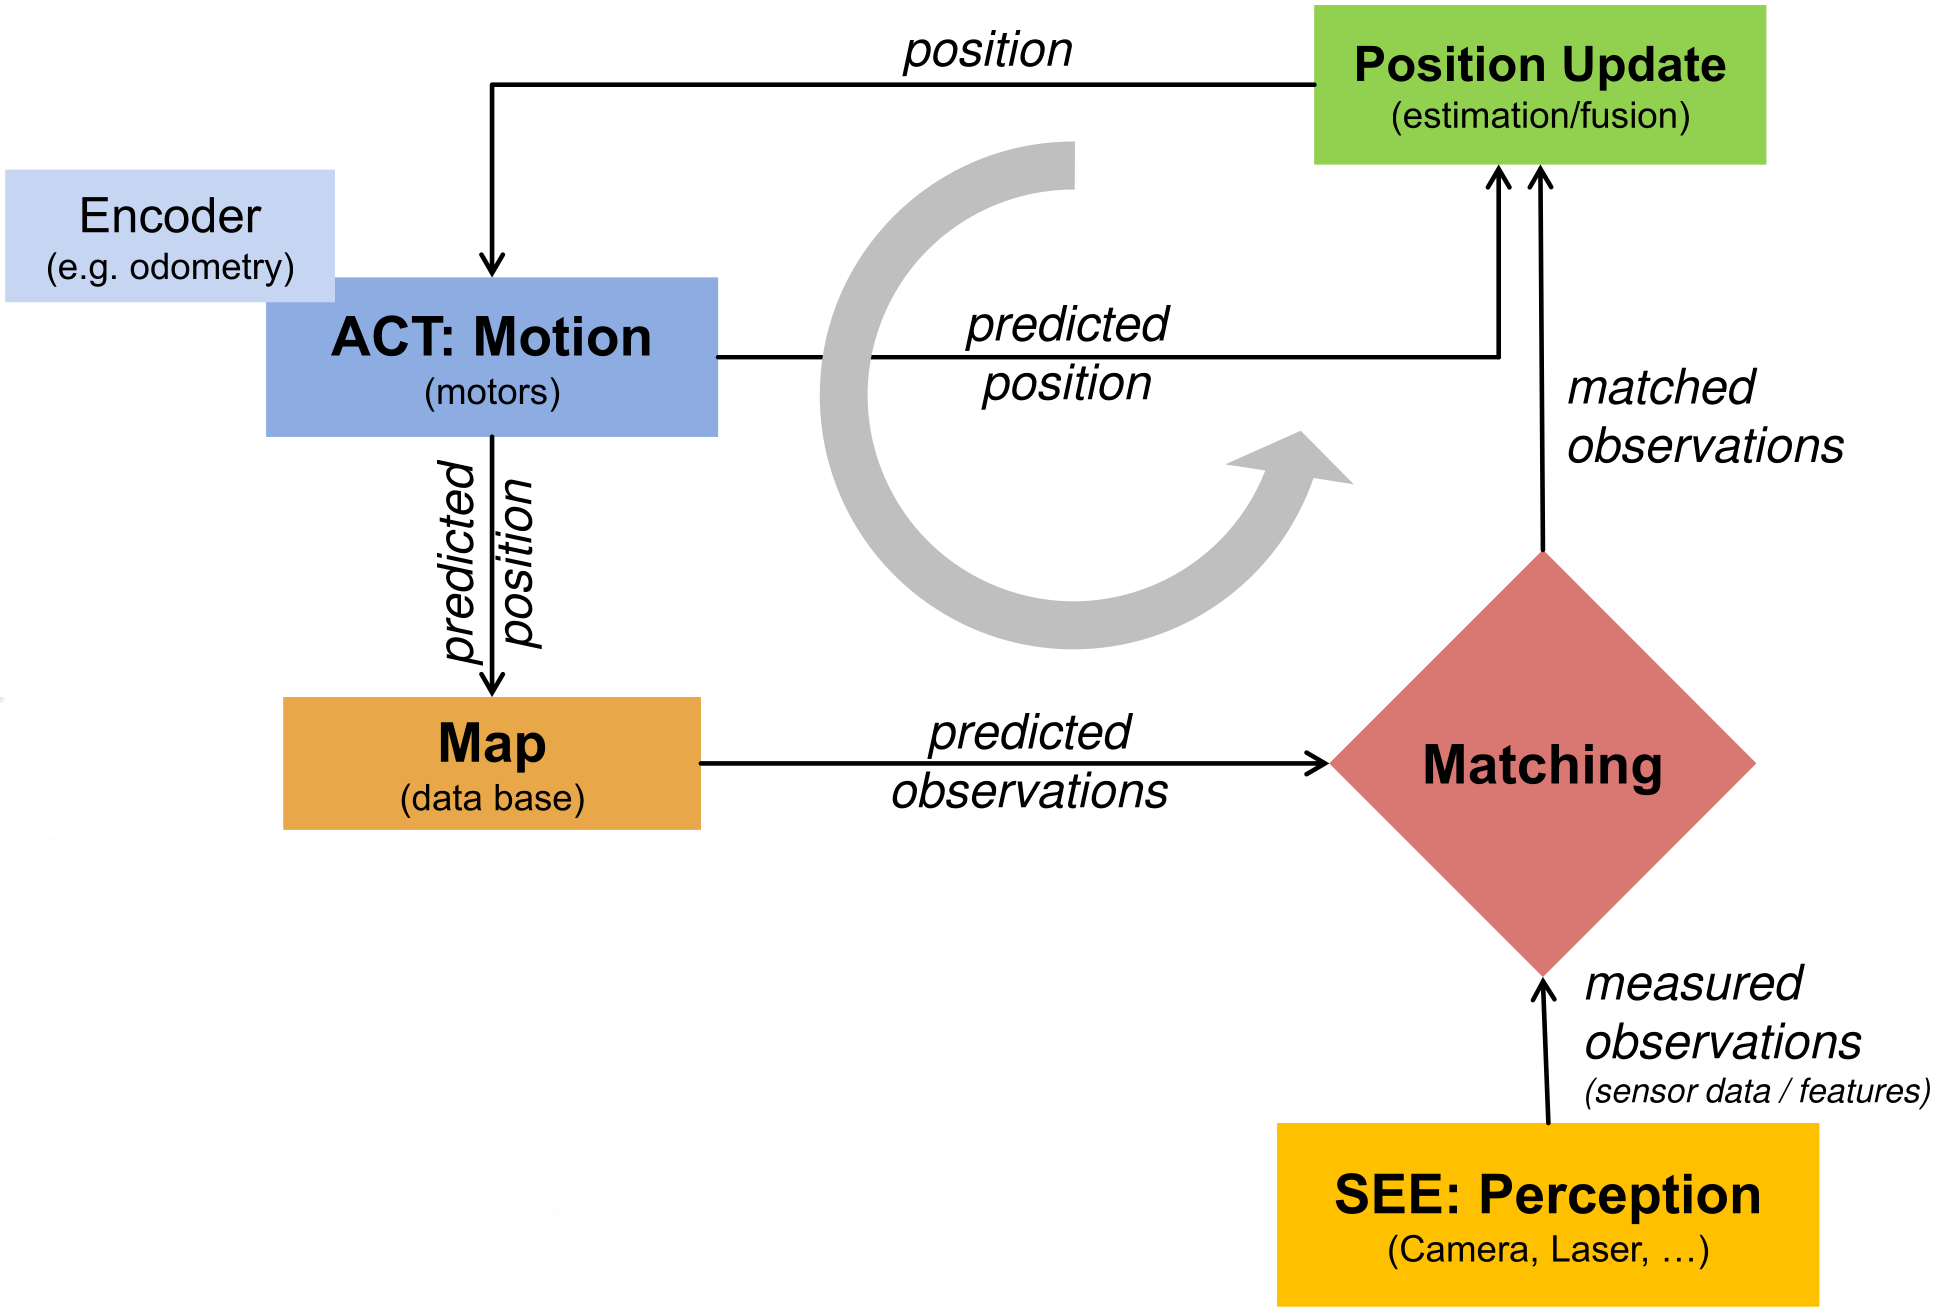
\includegraphics[width=\linewidth]{./Figures/05_LocalisationCycle.png}

\subsubsection{Markov Localization}
\begin{itemize}
    \ides{Solves:}
        \begin{itemize*}
            \item Global localization
            \item Position tracking
            \item Kidnapped robot
        \end{itemize*}
    \item Discretized pose representation $x_t$
    \item $\text{bel}(x_t)$ is representation by arbitrary prob. density function
        \begin{itemize}
            \item Multiple hypotheses
        \end{itemize}
    \ides{Markov Assumption:} $\text{bel}(x_t) = p(x_t \mid x_0, u_{0 \to t}, z_{0 \to t}) = p(x_t \mid x_{t - 1}, u_t, z_t)$
    \ides{Steps:}
\end{itemize}
\begin{algorithmic}
    \FORALL{$x_t$}
        \STATE \textit{S1)} \textbf{ACT:} $\overline{\text{bel}}(x_t) = \sum_{x_{t-1}} p(x_t \mid u_t, x_{t - 1}) \text{bel}(x_{t-1})$
        \STATE \textit{S2)} \textbf{SEE:} $\text{bel}(x_t) = \eta p(z_t \mid x_t, M) \overline{\text{bel}}(x_t)$ with $\eta = \frac{1}{p(y)}$
    \ENDFOR
\end{algorithmic}
\begin{itemize}
    \icon Huge state space
    \icon Inefficient
    \ides{Improvements:}
        \begin{itemize*}
            \item Change of cell size
            \item Adaptive cell size
            \ides{Randomized Sampling:} Approximation of belief state by a representative subset of possible locations. Higher density around peak points
        \end{itemize*}
\end{itemize}

\subsubsection{Extended Kalman Filter (EKF) Localization}
\begin{itemize}
    \ides{Solves:}
        \begin{itemize*}
            \item Position tracking
        \end{itemize*}
    \item $\text{bel}(x_t)$, motion model and measurement model is represented by a normal distribution
        \begin{itemize}
            \item Single hypotheses
        \end{itemize}
    \ides{Steps:}
        \begin{itemize}
            \item[S1)] \textbf{Prediction Update}
                \begin{itemize}
                    \item New position: $\hat x_t = f(x_{t-1}, u_t)$
                    \item Position uncertainty: $\hat P_t = F_x P_{t-1} F_x^\transpose + F_u Q_t F_u^\transpose$
                    \item
                        \begin{itemize}
                            \ides{$\mathbf{P_{t - 1}}$:} Covariance of the previous state $x - 1$
                            \ides{$\mathbf{Q_t}$:} Covariance of motion model noise
                            \ides{$\mathbf{F_{x/u}}$:} Jacobian w.r.t. $x/u$
                        \end{itemize}
                \end{itemize}
            \item[S2)] \textbf{Measurement Update}
                \begin{itemize}
                    \item[1)] \textbf{Observation:} Obtain set of observation $z_t^i$ with covariance $R_t^i, i=1 \dots n$
                    \item[2)] \textbf{Measurement Prediction:} Predict feature observations $\hat z_t^j = h^j(\hat x_t, m^j)$ and compute its Jacobian $H^j$ w.r.t $\hat x_t$

                    \item[3)] \textbf{Matching:}
                        \begin{itemize}
                            \item Compute the innovation $v_t^{ij} = [z_t^i - \hat z_t^j]$
                            \item Compute the innovation covariance $\Sigma_{IN_t}^{ij} = H^j \hat P_t {H^j}^\transpose + R_t^i$
                            \item Find matches with a validation gate $g$
                                \begin{itemize}
                                    \item Mahalanobis distance: ${v_t^{ij}}^\transpose (\Sigma_{IN_t}^{ij})^{-1} v_t^{ij} \le g^2$
                                \end{itemize}
                        \end{itemize}
                    \item[4)] \textbf{Estimation:}
                        \begin{itemize}
                            \item Stack validated observations into $z_t$, corresponding innovations into $v_t$, measurement Jacobians into $H_t$ and $R_t = \mathrm{diag}(R_t^i)$
                            \item Compute composite innovation covariance $\Sigma_{IN_t}$
                            \item For each match, update position estimate $x_t = \hat x_t + K_t v_t$
                            \item For each match, update covariance $P_t = \hat P_t - K_t \Sigma_{IN_t}K_t^\transpose$
                                \begin{itemize}
                                    \ides{Kalman Gain:} $K_t = \hat P_t H_t^\transpose (\Sigma_{IN_t})^{-1}$
                                \end{itemize}
                        \end{itemize}
                \end{itemize}
        \end{itemize}
    \ipro Precise
    \ipro Efficient
    \icon Robot may get lost
\end{itemize}

\subsection{Simultaneous Localization and Mapping (SLAM)}
\begin{itemize}
    \item Create map and localize in parallel only using proprioceptive and exteroceptive sensor data
    \ides{Terminology:}
        \begin{itemize*}
            \ides{$\mathbf{x_t}$:} robot location at time $t$
            \ides{$\mathbf{X_t}$}$=\{x_0, x_1, \dots, x_t\}$ robot path till time $t$
            \ides{$\mathbf{u_t}$:} motion between $t-1$ and $t$
            \ides{$\mathbf{U_t}$}$=\{u_0, u_1, \dots, u_t\}$ sequence of relative motions till time $t$
            \ides{$\mathbf{z_t}$:} landmark observation at time $t$
            \ides{$\mathbf{Z_t}$}$=\{z_0, z_1, \dots, z_t\}$ sequence of landmark observations till time $t$
            \ides{$\mathbf{z_t}$:} exteroceptive sensor reading (observation) at time $t$
            \ides{$\mathbf{M}$}$= \{m_0, m_1, \dots, m_{n-1}\}$ true map of the environment with $n$ landmarks
        \end{itemize*}
    \ides{Full SLAM:} Reconstruct full path $p(X_t, M \mid Z_t, U_t)$
    \ides{Online SLAM:} Reconstruct current position $p(x_t, M \mid Z_t, U_t)$
    \ides{Approaches:}
        \begin{itemize}
            \ides{Full Graph Optimisation}
                \begin{itemize}
                    \item Eliminate observations and control inputs
                    \item Solve for constraints between poses and landmarks
                    \ipro Finds globally consistent solution
                    \ipro Trajectories can be very smooth
                    \icon Sparsify graph for real-time application
                    \\ 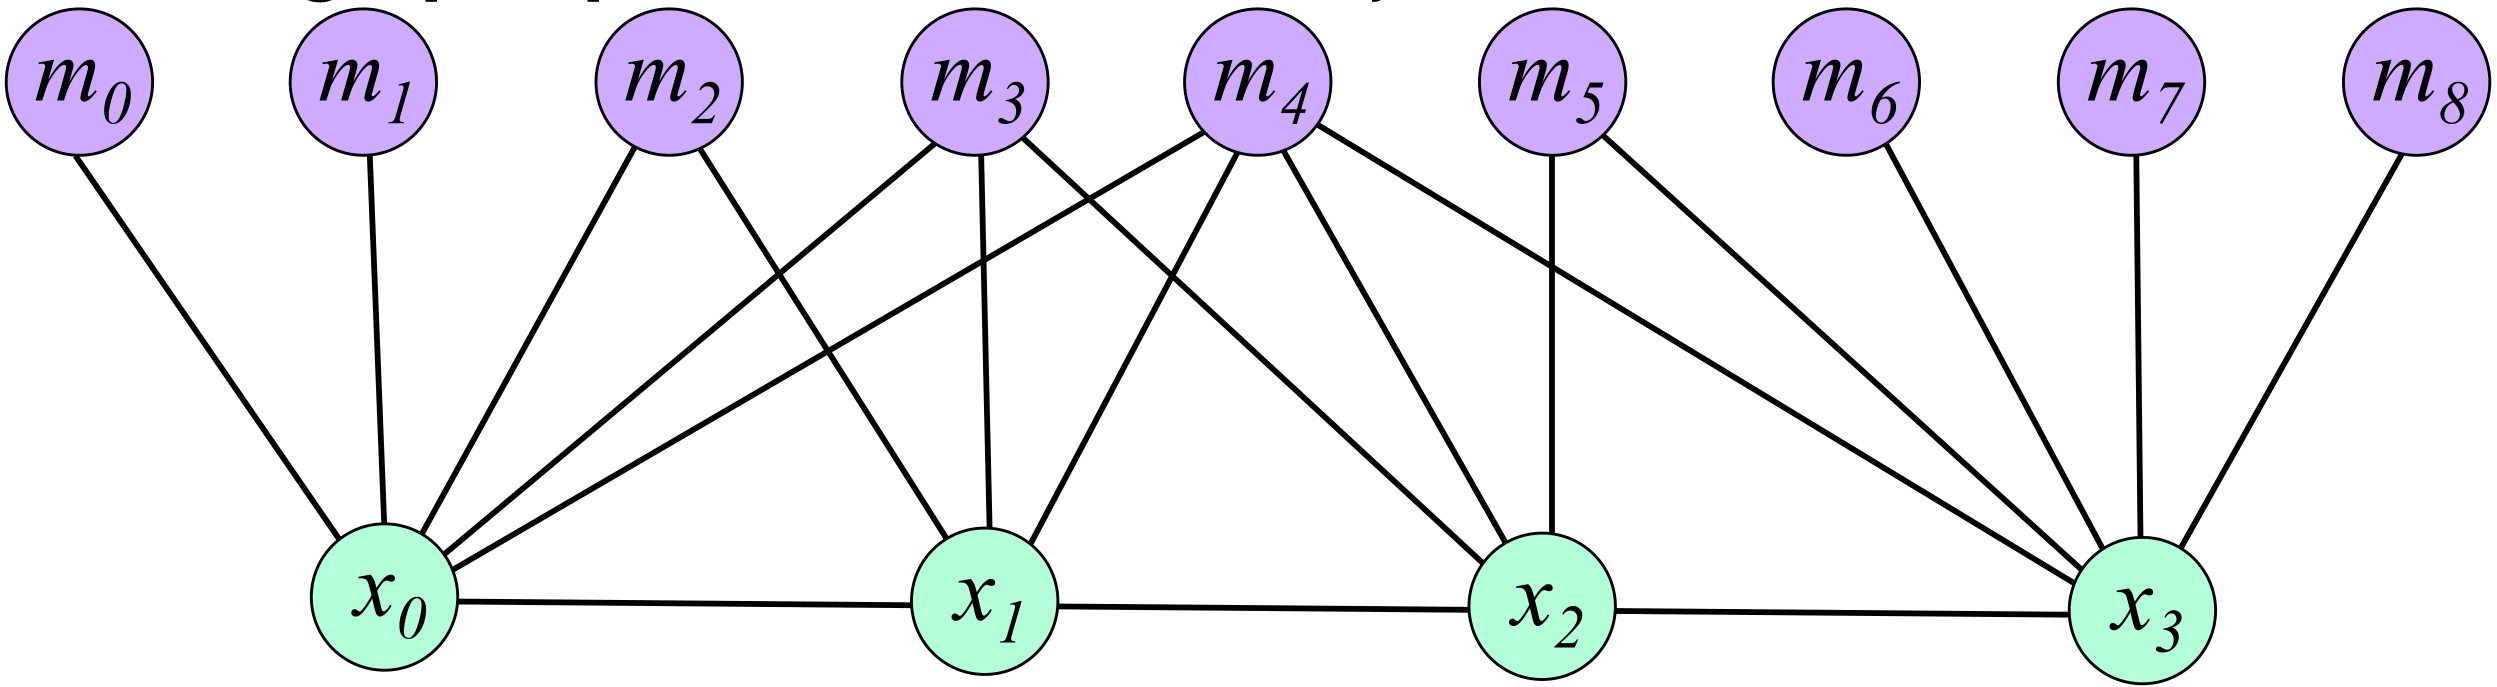
\includegraphics[width=\linewidth]{./Figures/05_SLAM_FullGraphOptimisation.png}
                \end{itemize}
            \ides{Key Frames}
                \begin{itemize}
                    \item Retain most representative poses and their dependency links
                    \item Optimize resulting graph
                    \item Example: PTAM, OKVIS, ORB-SLAM
                    \\ 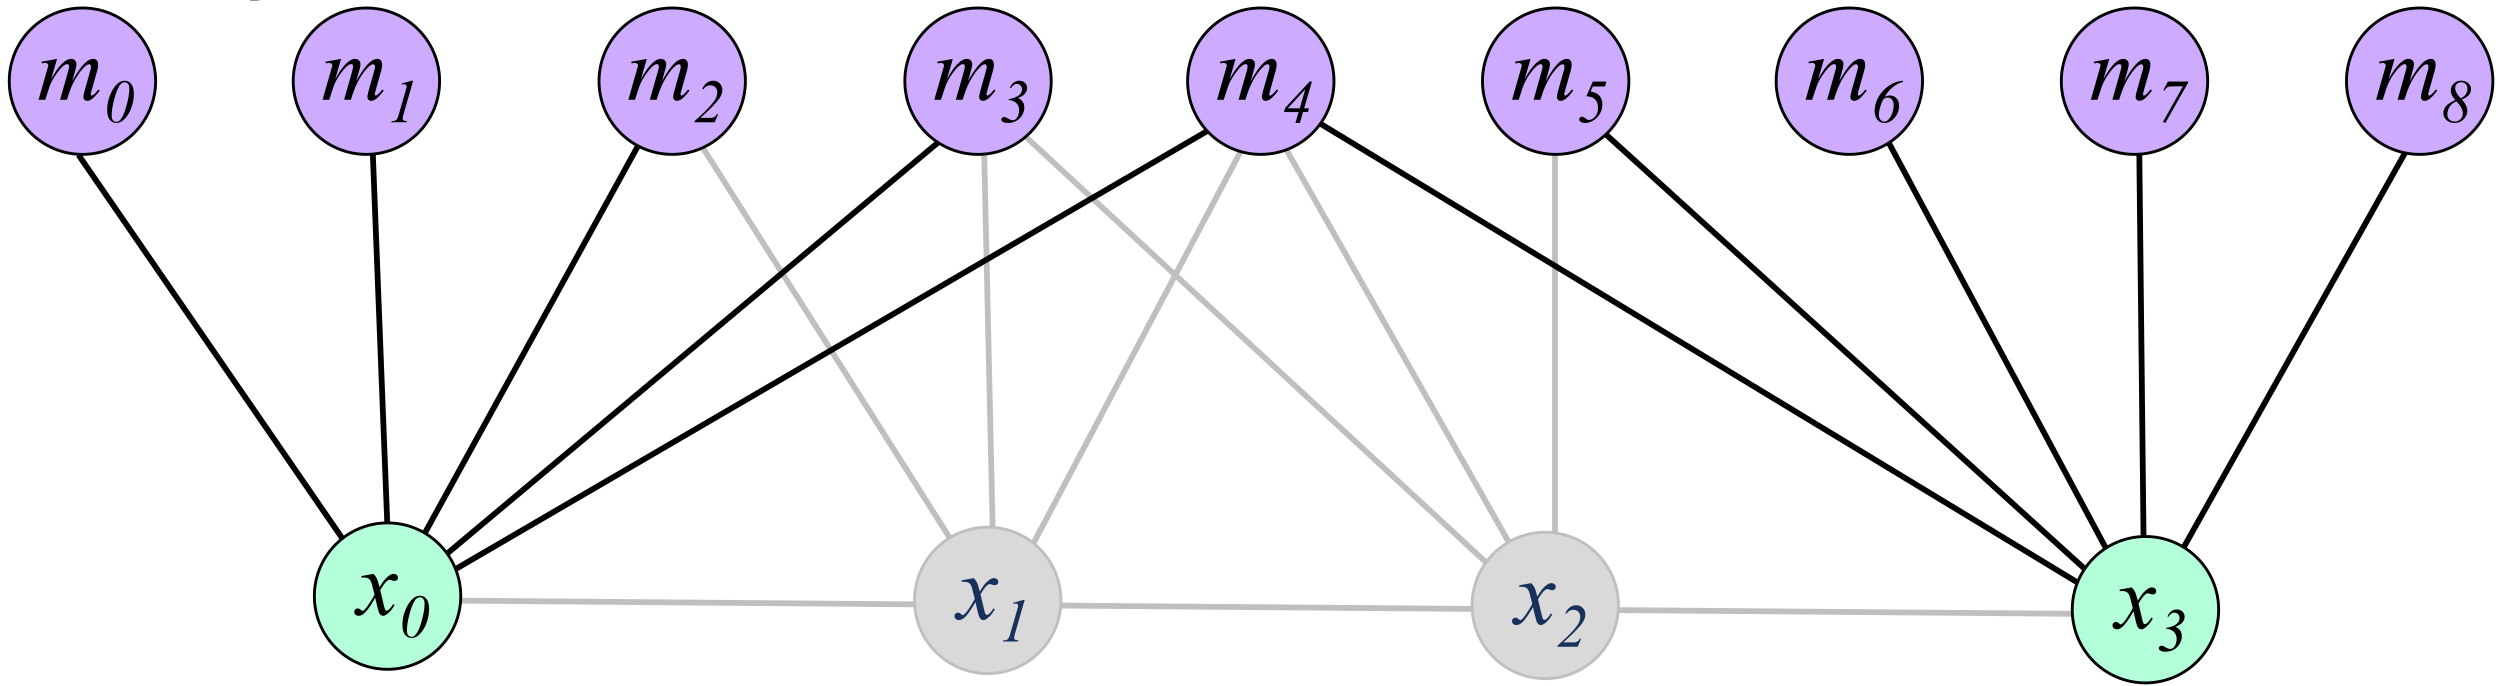
\includegraphics[width=\linewidth]{./Figures/05_SLAM_KeyFrames.png}
                \end{itemize}
            \ides{Filtering}
                \begin{itemize}
                    \item Summarize all experience w.r.t. last pose
                    \item Done using state vector and covariance matrix
                    \item Example: MonoSLAM, FastSLAM
                    \\ 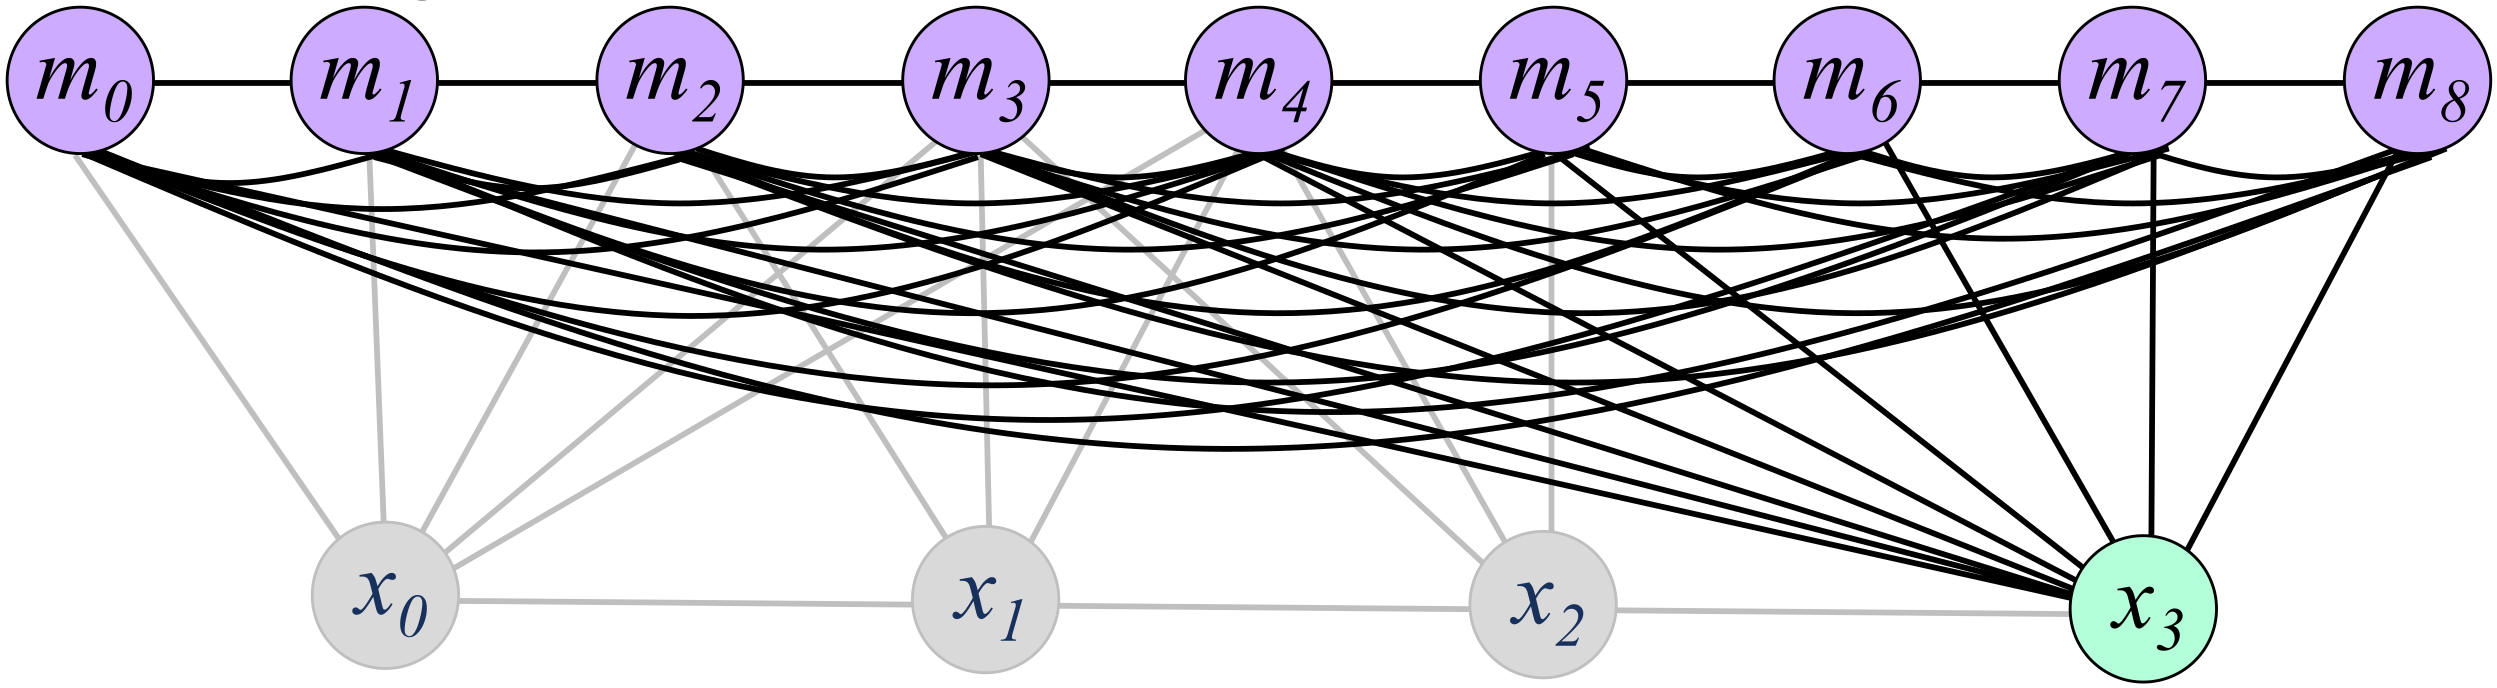
\includegraphics[width=\linewidth]{./Figures/05_SLAM_Filtering.png}
                \end{itemize}
        \end{itemize}
\end{itemize}

\subsubsection{EKF SLAM}
\begin{itemize}
    \item Example of filtering
    \item Summarizes past experience:
        \begin{itemize}
            \item Extended state vector $y_t =
                \begin{bmatrix}
                    x_t,  m_1, \cdots, m_{n-1}
                \end{bmatrix}^\transpose$
            \item Corresponding covariance $P_{y_t} =
                \begin{bmatrix}
                    P_{xx} & \cdots & P_{xm_{n-1}} \\
                    \vdots & \ddots & \vdots \\
                    P_{m_{n-1}x} & \cdots & P_{m_{n-1}m_{n-1}} \\
                \end{bmatrix}$
        \end{itemize}
    \item[S1)] \textbf{Prediction:}
        \begin{itemize}
            \item According to EKF equations
                \begin{itemize}
                    \item $\hat y_t =
                        \begin{bmatrix}
                          \hat x_t \\
                          m_i
                        \end{bmatrix} =
                        \begin{bmatrix}
                          f(x_{t-1}, u_t) \\
                          \mathbf 0
                        \end{bmatrix}$
                    \item $\hat P_{y_t} = F_y P_{y_{t-1}}F_y^\transpose + F_uQ_tF_u^\transpose$
                \end{itemize}
        \end{itemize}
    \item[S2)] \textbf{Measurement:}
        \begin{itemize}
            \item Measurement model $\hat z_i=h_i(\hat x_t, m_i)$ as in EKF localization
        \end{itemize}
    \item[S3)] \textbf{Update:}
        \begin{itemize}
            \item Update the state with actual observations $Z_{n-1}$:
            \item $y_t = \hat y_t + K_t (Z_{n-1} - h_{0:n-1}(\hat x_t, M_{n-1}))$
            \item $P_{y_t} = \hat P_{y_t} - K_t \Sigma_{IN} K_t^\transpose$
            \item Where
                \begin{itemize*}
                    \item $\Sigma_{IN} = H \hat P_{y_t} H^\transpose + R$
                    \item Kalman gain $K_t = \hat P_{y_t} H (\Sigma_{IN})^{-1}$
                \end{itemize*}
        \end{itemize}
    \item Initially, the covariance matrix is sparse (features are uncorrolated)
    \item After some time the covariance matrix becomes more dense
    \ides{MonoSLAM}
        \begin{itemize}
            \item EKF SLAM implementation
            \item Only one camera $\implies$ no proprioceptive data $\implies$ custom motion model
            \ides{Constant Velocity Motion Model}\\
                $f_v =
                \begin{bmatrix}
                  \mathbf r_\mathrm{new}^W \\
                  \mathbf q_\mathrm{new}^{WR} \\
                  \mathbf v_\mathrm{new}^W \\
                  \mathbf \omega_\mathrm{new}^W
                \end{bmatrix} =
                \begin{bmatrix}
                  \mathbf r^W + (\mathbf v^W + \mathbf V^W)\Delta t \\
                  \mathbf q^{WR} \times \mathbf q((\omega^W+\mathbf\Omega^W)\Delta t)\\
                  \mathbf v^W + \mathbf V^W\\
                  \mathbf \omega^W + \mathbf \Omega^W
                \end{bmatrix}$
            \item Unknown linear and angular accelerations cause a velocity impulse in each time step:\\
                $n =
                \begin{bmatrix}
                    \mathbf V^W\\
                    \mathbf \Omega^W
                \end{bmatrix} =
                \begin{bmatrix}
                    \mathbf a^W\Delta t\\
                    \mathbf \alpha^W\Delta t
                \end{bmatrix}$
        \end{itemize}
    \ides{Challenges}
        \begin{itemize*}
            \item Robust local motion estimation
            \item Mapping and loop-closure detection
            \item Map management and optimisation
            \item Sensitivity to incorrect data associations
            \item Tradeoff between efficiency and precision
            \item Dynamic objects
            \item Collaborative exploration
        \end{itemize*}
\end{itemize}

%! TEX root = ./main.tex

\section{Planning}
\begin{itemize}
    \ides{Completeness:} A robot system is complete iff for all possible problems, when a solution trajectory exists, the system will find it
\end{itemize}
\subsection{Path Planning}
\begin{itemize}
    \ides{Problem:} Find path in the physical space from the initial position to the goal position avoiding obstacles
    \ides{Workspace:} Physical area where the robot moves
    \ides{Configuration Space $C$:} $k$-dimensional space representing all configurations (position, rotations etc.) of a robot:
        \begin{itemize*}
            \item Occupied areas $O$
            \item Free areas $F = C \setminus O$
        \end{itemize*}
\end{itemize}

\subsubsection{Graph Search}
\begin{itemize}
    \ides{Idea:} Search path in connectivity graph of free space
    \item Consists of two steps
    \item[1)] \textbf{Graph Construction}
        \begin{itemize}
            \ides{Visibility Graph}
                \begin{itemize}
                    \item
                        \begin{itemize}
                            \item Polygonal configuration space
                            \item Robot is a point $\implies$ enlarge obstacles
                            \item Connect corners which ``see'' each other
                        \end{itemize}
                    \ipro Gives shortest path
                    \icon Complexity depends on number of obstacles
                    \icon Path is close to obstacles
                    \icon Does not consider robot motion constraints
                \end{itemize}
            \ides{Voroni Diagram}
                \begin{itemize}
                    \item
                        \begin{itemize}
                            \item For each point in free space compute the distance to the nearest obstacle
                            \item Points which are equidistant to two obstacles for edges
                        \end{itemize}
                    \ipro Maximizes distance to obstacles
                    \ipro Can do the process in reverse. Robot in unknown environment creates diagram by moving on unknown veroni edges
                    \icon Not optimal
                    \icon Does not consider robot motion constraints
                \end{itemize}
            \ides{Exact Cell Decomposition}
                \begin{itemize}
                    \item
                        \begin{itemize}
                            \item Draw lines according to obstacle geometry
                            \item Each filed is in either $F$ or $O$
                            \item Create connectivity graph from cells in $F$
                        \end{itemize}
                    \item Assumes: precise position in $F$ does not matter
                        \icon Complexity depends on number and complexity of obstacles
                \end{itemize}
            \ides{Approximate Cell Decomposition}
                \begin{itemize}
                    \item
                        \begin{itemize}
                            \item Put grid over map
                            \item Each cell is either in $O$ or $F$
                            \item Create connectivity graph from cells in $F$
                        \end{itemize}
                        \ides{Fixed-Size:} Grid has fixed size
                        \ides{Variable-Size:} Recursively split partially occupied cells into $4$ new cells
                        \icon Loss of narrow passages
                \end{itemize}
            \ides{Lattice Graph}
                \begin{itemize}
                    \item
                        \begin{itemize}
                            \item Overlay space with custom edges/curves
                            \item Each cell is either in $O$ or $F$
                            \item Create connectivity graph from cells in $F$
                        \end{itemize}
                    \item Cell decomposition is a special case of it
                    \ipro Great freedom
                \end{itemize}
        \end{itemize}
    \item[2)] \textbf{Graph Search}
        \begin{itemize}
            \item Expected cost from start to goal via node $n$: $f(n) = \underbrace{g(n)}_{\text{cost so far}} + \epsilon \underbrace{h(n)}_{\substack{\text{cost to go} \\ \text{heuristic}}}$
            \ides{Breath-First Search (BFS)}
                \begin{itemize}
                    \item Nodes expanded according to FIFO queue and closed list
                    \item Solution is optimal for uniform edge cost
                    \item $\bigO(|V| + |E|)$
                    \ipro First solution found is optional
                    \item Greedy backtracking of solution
                    \ides{BF(Graph G, Node Start, Node Goal)}
                        \begin{algorithmic}
                            \STATE FIFO.push(Start)
                            \WHILE{FIFO not empty}
                                \STATE Node current $\leftarrow$ FIFO.pop()
                                \IF{current $==$ Goal}
                                    \RETURN SUCCESS
                                \ENDIF
                                \STATE visited.push(current)
                                \STATE Nodes next = getNeighbours(current)
                                \FORALL{next $\notin$ visited}
                                    \STATE FIFO.push(next)
                                \ENDFOR
                            \ENDWHILE
                            \RETURN FAILURE
                        \end{algorithmic}
                \end{itemize}
            \ides{Depth-First Search (DFS)}
                \begin{itemize}
                    \item Nodes expanded according to LIFO queue and closed list
                    \ipro Better space complexity
                    \item $\bigO(|V| + |E|)$
                    \icon First solution found may not be optional
                    \item Greedy backtracking of solution
                    \ides{DF:} Same as BF but using LIFO
                \end{itemize}
            \ides{Dijkstra's Algorithm}
                \begin{itemize}
                    \item Nodes expanded according to Min-Heap (on $g(n)$) and closed list
                    \item Positive edge cost
                    \item $\bigO(|V| \log(|V|) + |E|)$
                    \item Often computed from the goal position to get all distances to the goal
                    \ipro First solution found is optional
                    \item Greedy backtracking of solution
                    \ides{Dijkstra(Graph G, Node Start, Node Goal)}
                        \begin{algorithmic}
                            \STATE MIN-HEAP.push(Start)
                            \WHILE{MIN-HEAP not empty}
                                \STATE Node current $\leftarrow$ MIN-HEAP.pop()
                                \IF{current $==$ Goal}
                                    \RETURN SUCCESS
                                \ENDIF
                                \STATE visited.push(current)
                                \STATE Nodes next = getNeighbours(current)
                                \FORALL{next $\notin$ visited}
                                    \STATE MIN-HEAP.push(next)
                                \ENDFOR
                            \ENDWHILE
                            \RETURN FAILURE
                        \end{algorithmic}
                \end{itemize}
            \ides{$\mathbf{A^*}$}
                \begin{itemize}
                    \item Nodes expanded according to Min-Heap (on $f(n)$) and closed list
                    \item Heuristic function guides search
                        \begin{itemize}
                            \item Must underestimate the distance
                            \item Often $h(n) =$ Distance from $n$ to goal
                        \end{itemize}
                    \item Positive edge cost
                    \item Good for single source shortest path
                    \item Runtime depends on chosen $h(n)$
                    \ipro First solution found is optional
                    \ipro Very efficient if we are ok finding a suboptimal solution
                        \begin{itemize}
                            \item Done if $\epsilon > 1$
                        \end{itemize}
                    \item Greedy backtracking of solution
                    \ides{A-Star(Graph G, Heur H, Node Start, Node Goal)}
                        \begin{algorithmic}
                            \STATE HEUR-MIN-HEAP.push(Start)
                            \WHILE{HEUR-MIN-HEAP not empty}
                                \STATE Node current $\leftarrow$ HEUR-MIN-HEAP.pop()
                                \IF{current $==$ Goal}
                                    \RETURN SUCCESS
                                \ENDIF
                                \STATE visited.push(current)
                                \STATE Nodes next = getNeighbours(current)
                                \FORALL{next $\notin$ visited}
                                    \STATE HEUR-MIN-HEAP.push(next)
                                \ENDFOR
                            \ENDWHILE
                            \RETURN FAILURE
                        \end{algorithmic}
                \end{itemize}
            \ides{Rapidly Exploring Random Trees (RRTs)}
                \begin{itemize}
                    \item Grows randomized tree
                    \item Selects random points and connects it to closest point of the tree using a new branch
                    \item Most likely returns suboptimal solution
                    \item Probabilistically complete
                    \ides{RRT(Node Start, Node Goal, System Sys, Environment Env)}
                        \begin{algorithmic}
                            \STATE Graph.init(Start)
                            \WHILE{Graph.size() $\le$ threshold}
                                \STATE Node rand = random()
                                \STATE Node near = Graph.nearest(rand)
                                \STATE \textbf{try}
                                \STATE $\quad$ Node new = Sys.propagate(near, rand)
                                \STATE $\quad$ Graph.addNode(new)
                                \STATE $\quad$ Graph.addEdge(near, new)
                                \STATE \textbf{end try}
                            \ENDWHILE
                            \RETURN FAILURE
                        \end{algorithmic}
                \end{itemize}
        \end{itemize}
\end{itemize}

\subsubsection{Potential Field Planning}
\begin{itemize}
    \ides{Idea:} Robot follows gradient of potential field
    \item Global
    \item Implicit incorporation of basic system models
    \ides{Local Potential Fields}
        \begin{itemize}
            \ides{Potential Field:} $U(q) = \underbrace{U_{\text{att}}(q)}_{\text{attractive}} + \underbrace{U_{\text{rep}}(q)}_{\text{repulsive}}$
            \item $U_{\text{att}}(q) = \frac{1}{2} k_{\text{att}} (q - q_{\text{goal}})^2$
            \item $U_{\text{rep}}(q) =
\begin{cases}
    \frac{1}{2} k_{\text{rep}}(\frac{1}{\rho(q)} - \frac{1}{\rho_{\text{lim}}})^2 & \text{if } \rho(q) \ge \rho_{\text{lin}}\\
    0 & \text{otherwise}
\end{cases}$
            \item
                \begin{itemize*}
                    \ides{$\mathbf{\rho(q)}$:} Min distance between $q$ and the closest obstacle
                    \ides{$\mathbf{\rho_{\text{lim}}}$:} Distance of influence of obstacle
                    \ides{$\mathbf{k_{\text{att/rep}}}$:} Scaling factor
                \end{itemize*}
            \item Robot follows force $F(q) = -\bigtriangledown U(q)$
            \icon May get stuck in local minima
            \icon No incorporation of robot's dynamic constraints
        \end{itemize}
    \ides{Harmonic Potential Fields}
        \begin{itemize}
            \item Robots follows solution of Laplace Equation $\triangle U = \sum \frac{\partial^2 U}{\partial^2 q_i} = 0$
            \item Boundary is specified according to:
                \begin{itemize}
                    \ides{Neumann:}
                        \begin{itemize*}
                            \item Equidistant lines parallel to the obstacles
                            \icon Potentially small distance to the obstacle
                            \item $\frac{\partial U(q)}{\partial q} = g(q) = 0$
                        \end{itemize*}
                    \ides{Dirchlet:}
                        \begin{itemize*}
                            \item Obstacle boundaries have constant high potential
                            \item Goal has constant low potential
                            \item Close to obstacles, robot moves perpendicularly away from obstacle
                            \item $U(q) = f(q) = \text{const}$
                            \ipro Safe paths
                            \icon Long paths
                        \end{itemize*}
                \end{itemize}
            \ipro Absence of local minima
            \item Solved via discretization of the workspace into cells
            \item Euler approximation: $\bigtriangledown U(q)_i \approx \frac{U(q + \delta e_i) - U(q)}{\delta}$
            \item Iterative method: $U^{k+1}(q) = \frac{1}{2n} \sum_{i=1}^{n} (U^k(q + \delta e_i) + U^k(q - \delta e_i))$\\
                \begin{itemize*}
                    \ides{$\mathbf{n}$:} \# dimensions
                    \ides{$\mathbf{e_i}$:} unit vector
                \end{itemize*}
            \item Steps from iteration $i$ to $i+1$
                \begin{itemize}
                    \item[1)] Initialize cell values
                        \begin{itemize}
                            \ides{Dirchlet:} Set obstacles to $1$ and goal and all other cells to $0$
                        \end{itemize}
                    \item[2)] Update all cells except goal and obstacles
                        \begin{itemize}
                            \item[a)] Add up values of $4$ neighbouring cells
                            \item[b)] Scale sum by $2n$
                            \item[c)] Update cell values
                        \end{itemize}
                    \item[3)] Repeat 2 till convergence
                    \item[4)] Backtrack solution
                \end{itemize}
        \end{itemize}
\end{itemize}

\subsection{Obstacle Avoidance}
\begin{itemize}
    \item Function of current on optionally past sensor readings, its current and goal location
    \icon Prone to local minima
    \ipro Incorporate system model
    \ides{Dynamic Window Approach (DWA)}
        \begin{minipage}[b]{0.5\linewidth}
            \raggedright
            \begin{itemize}
                \item Assume: robot moves on circular arcs $(\nu, \omega)$
                \ides{Obstacle space $\mathbf{V_o}$:} Transformation of obstacles from workspace to input space
            \end{itemize}
        \end{minipage}
        \begin{minipage}[b]{0.45\linewidth}
            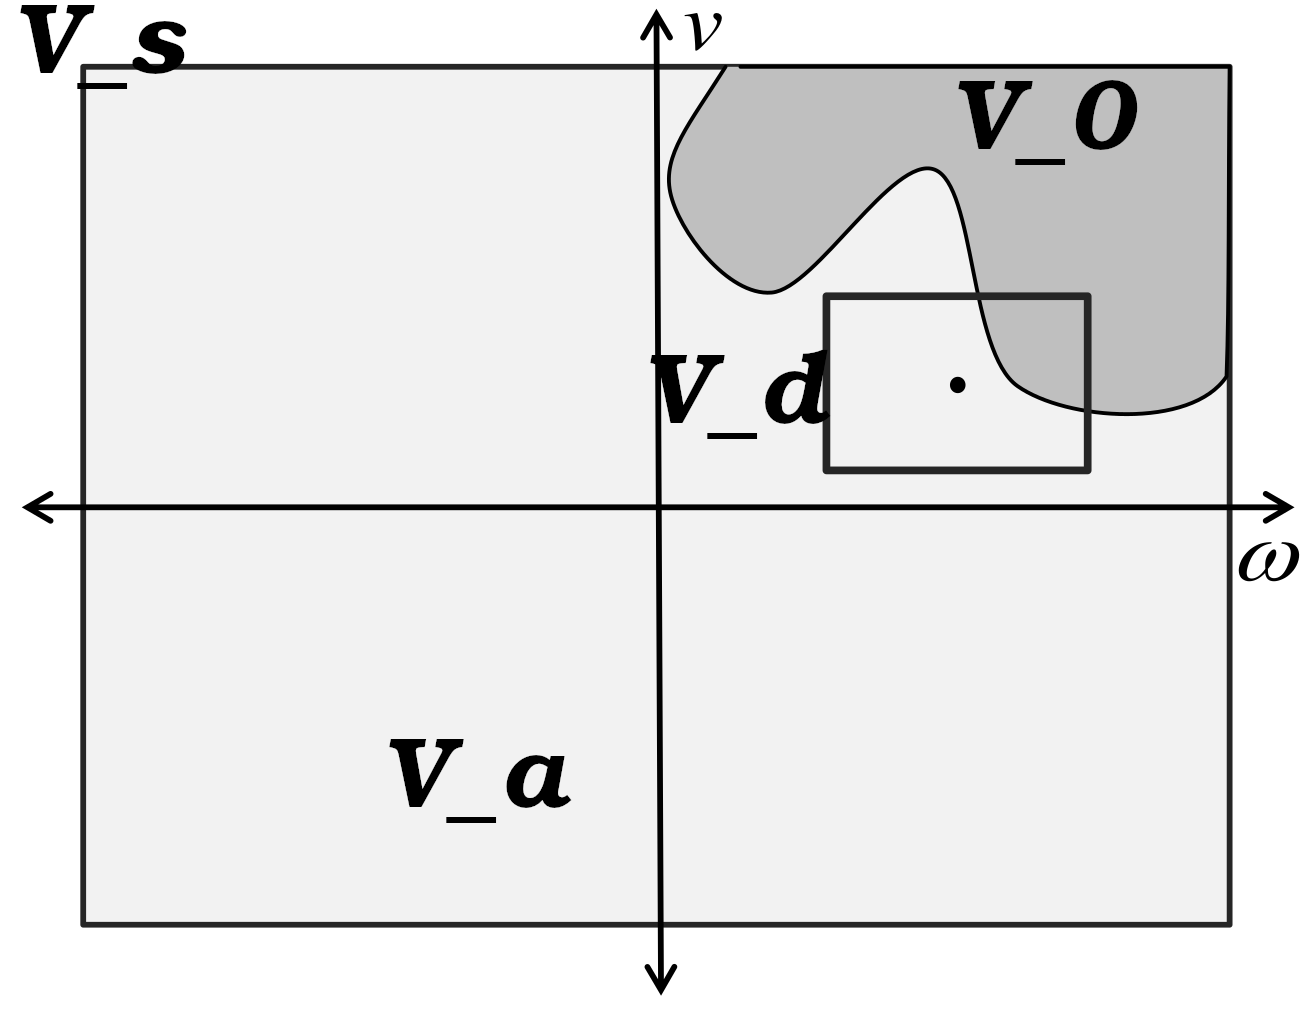
\includegraphics[width=0.97\linewidth]{./Figures/06_DWA.png}
        \end{minipage}
        \begin{itemize}
            \ides{Admissible space $\mathbf{V_a}$:} complement of $V_o$
            \ides{Static Window $\mathbf{V_s}$:} Configuration which are allowed by robot limits
            \ides{Dynamic Window $\mathbf{V_d}$:} Configuration which can be reached in one step
                \begin{itemize}
                    \item Centred around the current configuration
                \end{itemize}
            \ides{New configuration $\mathbf{V_r}$} $= V_a \cap V_s \cap V_d$
                \begin{itemize}
                    \item Selected which maximizes some objective function containing heading, distance to goal and velocity
                \end{itemize}
            \icon Not safe when obstacles are dynamic
        \end{itemize}
    \ides{Velocity Obstacles (VO)}
        \begin{minipage}[b]{0.5\linewidth}
            \raggedright
            \begin{itemize}
                \item Assume:
                    \begin{itemize*}
                        \item Robot moves on piece-wise linear curves
                        \item Robot is omnidirectional
                        \item Robot and obstacles are circular
                        \item Obstacles move at constant speed
                    \end{itemize*}
                \item Collision of robot and obstacle if $\lVert p_\text{RO} + \nu_R t \rVert < r_\text{R} + r_\text{O}$
            \end{itemize}
        \end{minipage}
        \begin{minipage}[b]{0.45\linewidth}
            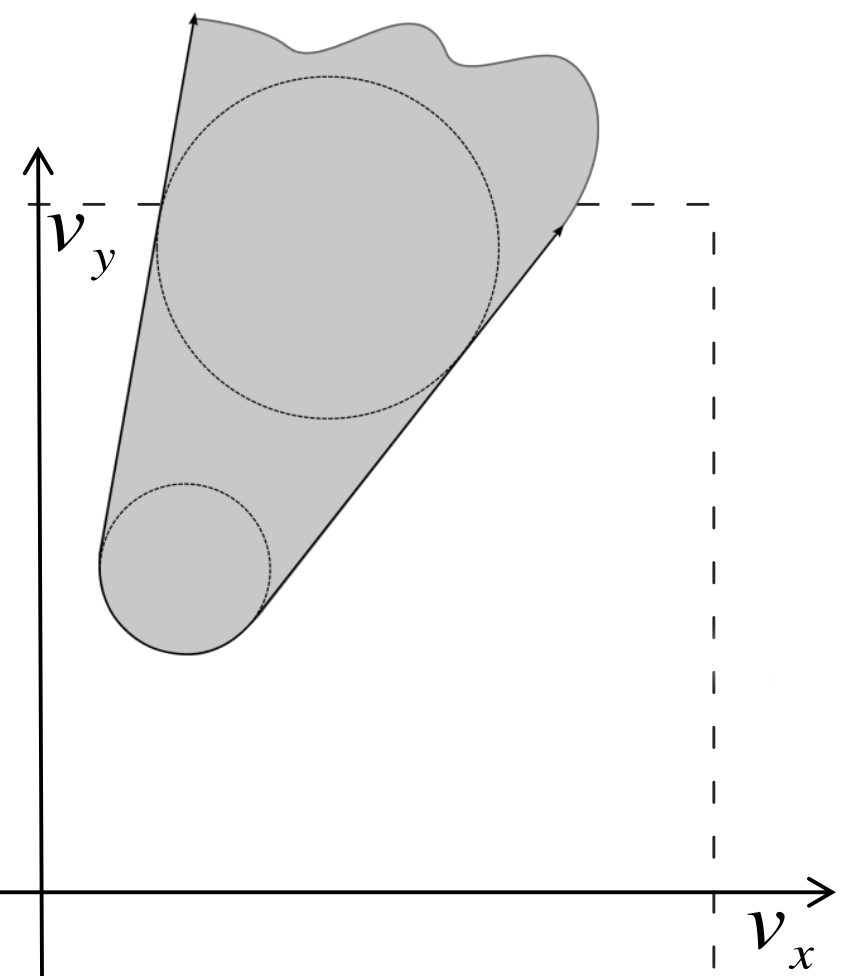
\includegraphics[width=0.97\linewidth]{./Figures/06_VO.png}
        \end{minipage}
        \begin{itemize}
            \ides{Velocity Obstacle:} Velocities in velocity space which lead to collisions in less than $\tau$ time
        \item $\text{VO}_\text{RO}^\tau = \bigcup_{0 \le t \le \tau} D(-\frac{p_\text{RO}}{t}, \frac{r_\text{RO}}{t})$
                \begin{itemize*}
                    \ides{$\mathbf{p_\text{RO}}$:} Relative position between robot and obstacle
                    \ides{$\mathbf{\text{VO}_\text{RO}}$:} Relative velocity between robot and obstacle
                    \ides{$\mathbf{r_\text{R/O}}$:} Radius of robot/obstacle
                    \ides{$\mathbf{D(x,y)}$:} Disc centred at $(x,y)$
                \end{itemize*}
            \item Multiple objects lead to multiple velocity obstacle regions
            \item Robot selects any velocity outside of the complement of VOs
            \icon Does not model interaction effects
    \end{itemize}
    \ides{Reciprocal Velocity Obstacles (RVO)}
        \begin{minipage}[b]{0.5\linewidth}
            \raggedright
            \begin{itemize}
                \item Assume:
                    \begin{itemize*}
                        \item Robot moves on piece-wise linear curves
                        \item Robot is omnidirectional
                        \item Robot and obstacles are circular
                        \item Fair behaviour of all agents
                    \end{itemize*}
            \item Identical to CO, but collision avoidance is shared between interaction agents
            \end{itemize}
        \end{minipage}
        \begin{minipage}[b]{0.45\linewidth}
            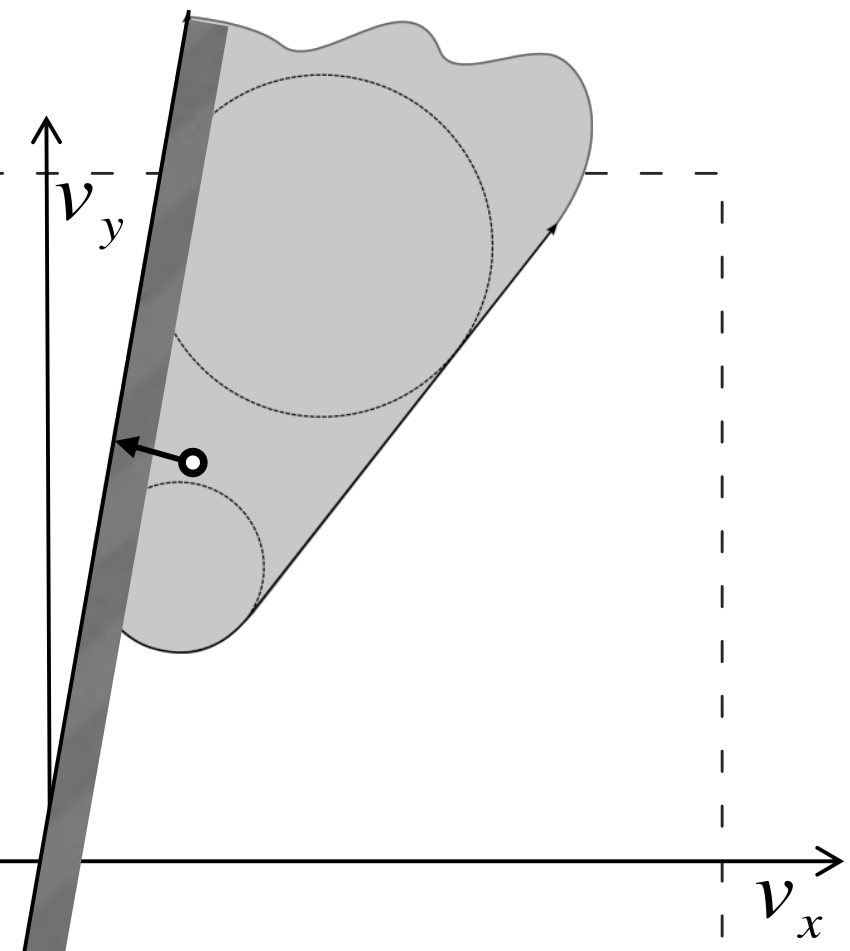
\includegraphics[width=\linewidth]{./Figures/06_RVO.png}
        \end{minipage}
        \begin{itemize}
            \item Operate in relative velocity space
            \item Linear constraints decides if obstacles are avoided to the left or right
                \begin{itemize}
                    \item Tangent to the boundary of the CO which is closer to the current velocity
                \end{itemize}
            \ides{Current relative velocity leads to collision:} Shift at least with half the velocity difference to the linear constraint
            \ides{Current relative velocity does not lead to collision:} Shift at most with half the velocity difference towards the linear constraint
        \end{itemize}
\end{itemize}

\end{document}
